\documentclass[10pt,a4paper]{article}
\usepackage[UTF8,fontset = windows]{ctex}
\setCJKmainfont[BoldFont=黑体,ItalicFont=楷体]{华文中宋}
\usepackage{amssymb,amsmath,amsfonts,amsthm,mathrsfs,dsfont,graphicx}
\usepackage{ifthen,indentfirst,enumerate,color,titletoc}
\usepackage{tikz}
\usepackage{multicol}
\usepackage{makecell}
\usepackage{longtable}
\usepackage{diagbox}
\usepackage{picinpar}
\usetikzlibrary{arrows,calc,intersections,patterns,decorations.pathreplacing,3d,angles,quotes,positioning}
\usepackage[bf,small,indentafter,pagestyles]{titlesec}
\usepackage[top=1in, bottom=1in,left=0.8in,right=0.8in]{geometry}
\renewcommand{\baselinestretch}{1.65}
\newtheorem{defi}{定义~}
\newtheorem{eg}{例~}
\newtheorem{ex}{~}
\newtheorem{rem}{注~}
\newtheorem{thm}{定理~}
\newtheorem{coro}{推论~}
\newtheorem{axiom}{公理~}
\newtheorem{prop}{性质~}
\newcommand{\blank}[1]{\underline{\hbox to #1pt{}}}
\newcommand{\bracket}[1]{(\hbox to #1pt{})}
\newcommand{\onech}[4]{\par\begin{tabular}{p{.9\textwidth}}
A.~#1\\
B.~#2\\
C.~#3\\
D.~#4
\end{tabular}}
\newcommand{\twoch}[4]{\par\begin{tabular}{p{.46\textwidth}p{.46\textwidth}}
A.~#1& B.~#2\\
C.~#3& D.~#4
\end{tabular}}
\newcommand{\vartwoch}[4]{\par\begin{tabular}{p{.46\textwidth}p{.46\textwidth}}
(1)~#1& (2)~#2\\
(3)~#3& (4)~#4
\end{tabular}}
\newcommand{\fourch}[4]{\par\begin{tabular}{p{.23\textwidth}p{.23\textwidth}p{.23\textwidth}p{.23\textwidth}}
A.~#1 &B.~#2& C.~#3& D.~#4
\end{tabular}}
\newcommand{\varfourch}[4]{\par\begin{tabular}{p{.23\textwidth}p{.23\textwidth}p{.23\textwidth}p{.23\textwidth}}
(1)~#1 &(2)~#2& (3)~#3& (4)~#4
\end{tabular}}

\begin{document}
\begin{enumerate}[1.]

%zmj1
\item 已知集合$A=\{1,2,3,4\}$, $B=\{2,4,6\}$, 则$A\cup B=$\blank{50}.
\item 不等式$\dfrac{x-2}{x+1}<0$的解集为\blank{50}.
\item 函数$y=\lg (x-1)+\dfrac 1{\sqrt {2-x}}$的定义域是\blank{50}.
\item 函数$y=\sin( \omega x-\dfrac{\pi}{3})$($\omega >0$)的最小正周期是$\pi$, 则$\omega =$\blank{50}.
\item 若函数$f(x)=\log_2(x+1)+a$的反函数的图像经过点$(4, 1)$, 则实数$a=$\blank{50}.
\item 已知幂函数$f(x)={x^\alpha}$的图像过点$(2,\dfrac{\sqrt 2}2)$, 则$f(x)$的定义域为\blank{50}.
\item 甲、乙两人从$5$门不同的选修课中各选修$2$门, 则甲、乙所选的课程中恰有$1$门相同的选法有\blank{50}种.
\item 设集合$M=\{x|x^2\le 1\}$, $N=\{b\}$, 若$M\cup N=M$, 则实数$b$的取值范围为\blank{50}.
\item 将函数$f(x)=\begin{vmatrix}
\sqrt 3 & \cos 2x  \\ 1 & \sin 2x  \end{vmatrix}$的图像向左平移$m$($m>0$)个单位, 所得图像对应的函数为偶函数, 则$m$的最小值为\blank{50}.
\item 如图, 在$\triangle ABC$中, $\angle B=45^\circ$, $D$是$BC$边上的一点, $AD=5$, $AC=7$, $DC=3$, 则$AB$的长为\blank{50}.
\begin{center}
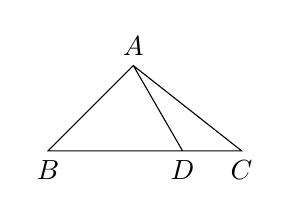
\begin{tikzpicture}[>=latex,scale = 0.25]
\draw (0,0) node [below] {$D$} coordinate (D);
\draw (3,0) node [below] {$C$} coordinate (C);
\draw (-2.5,{5*sqrt(3)/2}) node [above] {$A$} coordinate (A);
\draw ({-2.5-5*sqrt(3)/2},0) node [below] {$B$} coordinate (B);
\draw (B) -- (C) -- (A) -- cycle (A) -- (D);
\end{tikzpicture}
\end{center}
\item 若函数$f(x)$满足: \textcircled{1} 在定义域$D$内是单调函数; \textcircled{2} 存在$[a, b]\subseteq D$($a<b$), 使$f(x)$在$[a, b]$上的值域为$[-b, -a]$, 那么$y=f(x)$叫做对称函数. 现有$f(x)=\sqrt {1-x}-k$是对称函数, 则实数$k$的取值范围是\blank{50}.
\item 如图, 已知正三棱柱的底面边长为$2\text{cm}$, 高为$5\text{cm}$,
一质点自$A$点出发, 沿着三棱柱的侧面绕行两周到达$A_1$点的最短路线的长为\blank{50}$\text{cm}$.
\begin{center}
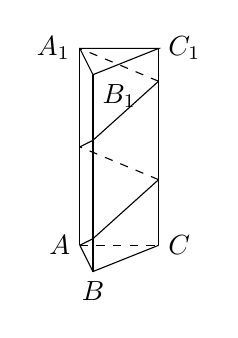
\begin{tikzpicture}[>=latex,scale = 0.5]
\draw (0,0,0) node [left] {$A$} coordinate (A);
\draw (2,0,0) node [right] {$C$} coordinate (C);
\draw (1,0,{sqrt(3)}) node [below] {$B$} coordinate (B);
\draw (A) -- (B) -- (C);
\draw (A) --++ (0,5) node [left] {$A_1$} coordinate (A1);
\draw (B) --++ (0,5) node [below right] {$B_1$} coordinate (B1);
\draw (C) --++ (0,5) node [right] {$C_1$} coordinate (C1);
\draw (A1) -- (B1) -- (C1) -- cycle;
\draw [dashed] (A) -- (C);
\draw (A) -- ($(B)!{1/6}!(B1)$) -- ($(C)!{1/3}!(C1)$)  ($(A)!0.5!(A1)$) -- ($(B)!{2/3}!(B1)$) -- ($(C)!{5/6}!(C1)$);
\draw [dashed] ($(C)!{1/3}!(C1)$) -- ($(A)!0.5!(A1)$) ($(C)!{5/6}!(C1)$) -- (A1);
\end{tikzpicture}
\end{center}
\item ``$x<2$''是``$x^2<4$''的\bracket{20}.
\twoch{充分非必要条件}{必要非充分条件}{充分必要条件}{既非充分又非必要条件}
\item 对任意向量$\overrightarrow a$、$\overrightarrow b$, 下列关系式中不恒成立的是\bracket{20}.
\twoch{$(\overrightarrow a+\overrightarrow b)^2=|\overrightarrow a+\overrightarrow b|^2$}{$(\overrightarrow a+\overrightarrow b)\cdot (\overrightarrow a-\overrightarrow b)=\overrightarrow a^2-\overrightarrow b^2$}{$|\overrightarrow a\cdot \overrightarrow b|\le|\overrightarrow a|\cdot|\overrightarrow b|$}{$|\overrightarrow a-\overrightarrow b|\le||\overrightarrow a|-|\overrightarrow b||$}
\item 设$m$、$n$为两条直线, $\alpha$、$\beta$为两个平面, 则下列命题中假命题是\bracket{20}.
\twoch{若$m\perp n$, $m\perp \alpha$, $n\perp \beta$, 则$\alpha \perp \beta$}{若$m\parallel n$, $m\perp \alpha$, $n\parallel \beta$, 则$\alpha \perp \beta$}{若$m\perp n$, $m\parallel \alpha$, $n\parallel \beta$, 则$\alpha \parallel \beta$}{若$m\parallel n$, $m\perp \alpha$, $n\perp \beta$, 则$\alpha \parallel \beta$}
\item 已知函数$y=f(x)$的定义域为$D$, $x_1,x_2\in D$. 关于$y=f(x)$ 的两个命题:\\
命题\textcircled{1}: 若当$f(x_1)+f(x_2)=0$时, 都有$x_1+x_2=0$, 则函数$y=f(x)$是$D$上的奇函数.\\
命题\textcircled{2}: 若当$f(x_1)<f(x_2)$时, 都有$x_1<x_2$, 则函数$y=f(x)$是$D$上的增函数.\\
下列判断正确的是\bracket{20}.
\twoch{\textcircled{1} 和\textcircled{2} 都是真命题}{\textcircled{1} 是真命题, \textcircled{2} 是假命题}{\textcircled{1} 和\textcircled{2} 都是假命题}{\textcircled{1} 是假命题, \textcircled{2} 是真命题}
\item 如图: 已知$AB\perp$平面$BCD$, $BC\perp CD$, $AD$与平面$BCD$所成的角为$30^\circ$, 且$AB=BC=2$.\\
(1) 求三棱锥$A-BCD$的体积;\\
(2) 设$M$为$BD$的中点, 求异面直线$AD$与$CM$所成角的大小(结果用反三角函数值表示).
\begin{center}
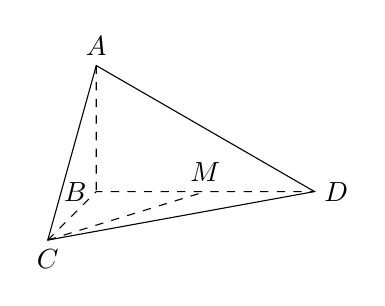
\begin{tikzpicture}[>=latex,scale = 0.8]
\draw (0,0,0) node [left] {$B$} coordinate (B);
\draw (0,2,0) node [above] {$A$} coordinate (A);
\draw (0,0,2) node [below] {$C$} coordinate (C);
\draw ({2*sqrt(3)},0,0) node [right] {$D$} coordinate (D);
\draw ($(B)!0.5!(D)$) node [above] {$M$} coordinate (M);
\draw [dashed] (C) -- (B) -- (D) (A) -- (B) (C) -- (M);
\draw (A) -- (C) -- (D) -- cycle;
\end{tikzpicture}
\end{center}
\item 已知$x\in \mathbf{R}$, 设$\overrightarrow m=(2\cos x, \sin x+\cos x)$, $\overrightarrow n=(\sqrt 3\sin x, \sin x-\cos x)$, 记函数$f(x)=\overrightarrow m\cdot \overrightarrow n$.\\
(1) 求函数$f(x)$取最小值时$x$的取值范围;\\
(2) 设$\triangle ABC$的角$A$, $B$, $C$所对的边分别为$a$, $b$, $c$, 若$f(C)=2$, $c=\sqrt 3$, 求$\triangle ABC$的面积$S$的最大值.
\item 如图, 某城市有一矩形街心广场$ABCD$, 如图. 其中$AB=4$百米, $BC=3$百米.现将在其内部挖掘一个三角形水池$DMN$种植荷花, 其中点$M$在边$BC$上, 点$N$在边$AB$上, 要求$\angle MDN=\dfrac{\pi}4$.
\begin{center}
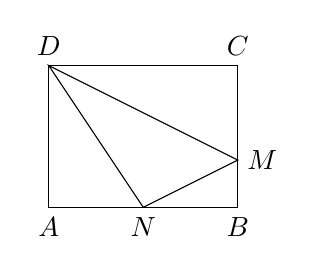
\begin{tikzpicture}[>=latex,scale = 0.6]
\draw (0,0) node [below] {$A$} coordinate (A) -- (4,0) node [below] {$B$} coordinate (B) -- (4,3) node [above] {$C$} coordinate (C) -- (0,3) node [above] {$D$} coordinate (D) -- cycle;
\draw (2,0) node [below] {$N$} coordinate (N) -- (4,1) node [right] {$M$} coordinate (M) -- (D) -- cycle;
\end{tikzpicture}
\end{center}
(1) 若$AN=CM=2$百米, 判断$\triangle DMN$是否符合要求, 并说明理由;\\
(2) 设$\angle CDM=\theta$, 写出$\triangle DMN$面积的$S$关于$\theta$的表达式, 并求$S$的最小值.
\item 已知数列$\{a_n\}$的前$n$项和为$S_n$, 且$a_1=1$, $a_2=a$.\\
(1) 若数列$\{a_n\}$是等差数列, 且$a_8=15$, 求实数$a$的值;\\
(2) 若数列$\{a_n\}$满足$a_{n+2}-a_n=2$($n\in \mathbf{N}^*)$, 且$S_{19}=19a_{10}$, 求证: 数列$\{a_n\}$是等差数列;
\item 已知函数$f(x)=2^x+k\cdot 2^{-x}$($x\in \mathbf{R}$).\\
(1) 判断函数$f(x)$的奇偶性, 并说明理由;\\
(2) 设$k>0$, 问函数$f(x)$的图像是否关于某直线$x=m$成轴对称图形, 如果是, 求出$m$的值; 如果不是, 请说明理由; (可利用真命题: ``函数$g(x)$的图像关于某直线$x=m$成轴对称图形''的充要条件为``函数$g(m+x)$是偶函数'')\\
(3) 设$k=-1$, 函数$h(x)=a\cdot 2^x-2^{1-x}-\dfrac 43a$, 若函数$f(x)$与$h(x)$的图像有且只有一个公共点, 求实数$a$的取值范围.


%zmj2
\item 设集合$A=\{x\in\mathbf{R}|0\le x\le 1\}$, $B=\{x\in \mathbf{R}|(x-1)(x-2)\le 0\}$, 则$A\cup B=$\blank{50}.
\item 函数$y=x^2$($x\ge 0$)的反函数为\blank{50}.
\item 若$0<\alpha<\pi$, $\cos\alpha=-\dfrac 13$, 则$\tan\alpha=$\blank{50}.
\item 复数$\dfrac{2+4\mathrm{i}}{1+\mathrm{i}}$的虚部为\blank{50}.
\item 若正方体的棱长为$1$, 则其外接球的体积为\blank{50}.
\item 已知函数$f(x)=\sin(3x+\varphi)$($-\dfrac\pi 2<\varphi<\dfrac\pi 2$)的图像关于直线$x=\dfrac \pi 4$对称, 则$\varphi=$\blank{50}.
\item 一个袋中装有同样大小、质量的$10$个球, 其中$2$个红球、$3$个蓝球、$5$个黑球. 经过充分混合后, 若从此袋中任意取出$4$个球, 则三种颜色的球均取到的概率为\blank{50}.
\item 若抛物线$y^2=8x$的准线与曲线$\dfrac{x^2}a+\dfrac{y^2}4=1$($a>0$)只有一个公共点, 则$a$的取值范围为\blank{50}.
\item 设函数$f(x)=\dfrac 1x-\lg x$, 则不等式$f(\dfrac 1x-1)<1$的解集为\blank{50}.
\item 若$\ln x$与$\ln y$的算术平均值为$1$, 则$\mathrm{e}^x$与$\mathrm{e}^y$的几何平均值的最小值为\blank{50}.
\item 正方形$ABCD$的边长为$4$, $O$是正方形$ABCD$的中心, 过中心$O$的直线$l$与边$AB$交于点$M$, 与边$CD$交于点$N$. $P$为平面上一点, 满足$2
\overrightarrow{OP}=\lambda \overrightarrow{OB}+(1-\lambda)\overrightarrow{OC}$, 则$\overrightarrow{PM}\cdot \overrightarrow{PN}$的最小值为\blank{50}.
\item 已知常数$b,c\in \mathbf{R}$, 若函数$f(x)=x+\dfrac bx+c$在区间$[1,+\infty)$上存在零点, 则$b^2+c^2$的取值范围为\blank{50}.
\item 曲线$y^2=9x$的准线方程是\bracket{20}.
\fourch{$x=4$}{$x=2$}{$x=-2$}{$x=-4$}
\item 设$x,y$均为实数, 且$\begin{vmatrix}x & 3 \\ 6 & 2 \end{vmatrix} - \begin{vmatrix} 1 & 4 \\ 5 & 7\end{vmatrix} = 7$, 则在以下各项中$(x,y)$的可能取值只能是\bracket{20}.
\fourch{$(2,1)$}{$(2,-1)$}{$(-1, 2)$}{$(-1, -2)$}
\item 已知垂直竖在水平地面上相距$20\text{m}$的两根旗杆的高分别为$10\text{m}$、$15\text{m}$, 地面上的动点$P$到两旗杆顶点的仰角相等, 则点$P$的轨迹是\bracket{20}.
\fourch{椭圆}{圆}{双曲线}{抛物线}
\item 已知常数$b,c\in \mathbf{R}$, 关于$x$的方程$x^2+b|x|+c=0$在复数集$\mathbf{C}$上给出下列两个结论: \textcircled{1} 存在$b,c$, 使得该方程有且只有$2$个共轭虚根; \textcircled{2} 存在$b,c$, 使得该方程有且只有$6$个互不相等的根, 则\bracket{20}.
\fourch{\textcircled{1}与\textcircled{2}均正确}{\textcircled{1}正确, \textcircled{2}不正确}{\textcircled{1}不正确, \textcircled{2}正确}{\textcircled{1}与\textcircled{2}均不正确}
\item 设常数$a\in \mathbf{R}$, 函数$f(x)=a\sin 2x+\cos(2\pi-2x)+1$.\\
(1) 若$a=\sqrt{3}$, 求$f(x)$的单调递增区间;\\
(2) 若$f(x)$为偶函数, 求$f(x)$的值域.
\item 设$\triangle ABC$的内角$A,B,C$所对的边分别为$a,b,c$, 满足$\sin A=\sqrt{3}\sin B$, $C=\dfrac\pi 6$.\\
(1) 若$ac=\sqrt{3}$, 求$\triangle ABC$的面积;\\
(2) 能否将$\triangle ABC$的边长按某种顺序排列为一个等比数列? 说明理由.
\item 某商场共有三层楼, 在其圆柱形空间内安装两部等长的扶梯I和II供顾客乘用. 如图, 一顾客自一楼点$A$处乘I到达二楼的点$B$处后, 沿着二楼面上的圆弧$BM$逆时针步行至点$C$处, 且$C$为圆弧$BM$的中点, 再乘II到达三楼的点$D$处. 设圆柱形空间三个楼面圆的中心分别为$O,O_1,O_2$, 半径为$8\text{m}$, 相邻楼层的间距$AB=4\text{m}$, 两部扶梯与楼面所成角的大小均为$\arcsin\dfrac 13$.
\begin{center}
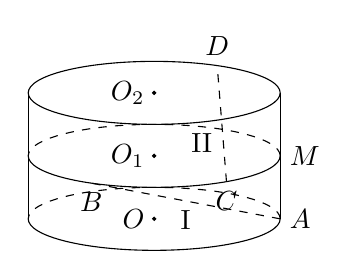
\begin{tikzpicture}[>=latex,scale = 0.2]
\filldraw (0,8) circle (0.1) node [left] {$O_2$};
\filldraw (0,4) circle (0.1) node [left] {$O_1$};
\filldraw (0,0) circle (0.1) node [left] {$O$};
\draw (0,8) ellipse (8 and 2);
\draw (8,4) arc (0:-180:8 and 2) (8,0) arc (0:-180:8 and 2);
\draw [dashed] (8,4) arc (0:180:8 and 2) (8,0) arc (0:180:8 and 2);
\draw (8,0) node [right] {$A$} coordinate (A) -- (8,4) node [right] {$M$} coordinate (M) -- (8,8);
\draw (-8,0) -- (-8,8);
\draw ({8*cos(-120)},{4+2*sin(-120)}) node [below] {$B$} coordinate (B);
\draw ({8*cos(-55)},{4+2*sin(-55)}) node [below] {$C$} coordinate (C);
\draw ({8*cos(60)},{8+2*sin(60)}) node [above] {$D$} coordinate (D);
\draw [dashed] (A) -- (B) node [midway, below] {I};
\draw [dashed] (C) -- (D) node [midway, below left] {II};
\end{tikzpicture}
\end{center}
(1) 求此顾客在二楼面上步行的路程;\\
(2) 求异面直线$AB$与$CD$所成角的大小(结果用反三角函数表示).
\item 已知曲线$\Gamma:x^2-y|y|=1$与$x$轴分别相交于$A,B$两点($A$在$B$的左侧), $\Gamma$与$y$轴相交于点$C$. 已知$F_1(-c,0)$, $F_2(c,0)$, $c>0$, $\triangle BCF_1$的面积为$\dfrac{1+\sqrt{2}}{2}$.\\
(1) 若过$F_2$的直线$l$与$\Gamma$有且仅有一个公共点, 直接写出$l$倾斜角的取值范围;\\
(2) 过点$B$作斜率存在的直线$m$交$\Gamma$于$P,Q$两点(异于点$B$), 且点$P$在第一象限, 求证: $P,Q$的横坐标之积为定值, 并求该定值;\\
(3) 在(2)的条件下, 当$\overrightarrow{F_1P}\cdot \overrightarrow{F_1Q}=3+2\sqrt{2}$时, 求$\dfrac{|AP|}{|AQ|}$的值.
\item 已知数列$\{a_n\}$满足$a_n\ne 0$恒成立.\\
(1) 若$a_na_{n+2}=ka_{n+1}^2$且$a_n>0$, 当$\{\lg a_n\}$成等差数列时, 求$k$的值;\\
(2) 若$a_na_{n+2}=2a_{n+1}^2$且$a_n>0$, 当$a_1=1$, $a_4=16\sqrt{2}$时, 求$\{a_n\}$的通项公式;\\
(3) 若$a_na_{n+2}=-\dfrac 12a_{n+1}a_{n+3}$, $a_1=-1$, $a_3\in [4, 8]$, $a_{2020}<0$, 求$a_1+a_2+\cdots+a_{2020}$的最大值.

%zmj3
\item 已知全集$U=\mathbf{R}$, 集合$A=\{x||x-1|>1\}$, $B=\{x|\dfrac{x-3}{x+1}<0\}$, 则$\complement _UA\cap B=$\blank{50}.
\item 已知幂函数的图像过点$(2,\dfrac 14)$, 则该幂函数的单调递增区间是\blank{50}.
\item 若$S_n$是等差数列$\{a_n\}$($n\in \mathbf{N}^*$): $-1,2,5,8,\cdots$的前$n$项和, 则$\displaystyle\lim_{n\to\infty}\dfrac{S_n}{n^2+1}=$\blank{50}.
\item 某圆锥体的底面圆的半径长为$\sqrt 2$, 其侧面展开图是圆心角为$\dfrac 23\pi$的扇形, 则该圆锥体的体积是\blank{50}.
\item 过点$P(-2,1)$作圆$x^2+y^2=5$的切线, 则该切线的点法向式方程是\blank{50}.
\item 函数$f(x)=\sqrt 3\sin x\cos x+\cos ^2x$的最大值为\blank{50}.
\item 若关于$x$、$y$的二元一次线性方程组$\begin{cases} a_1x+b_1y=c_1 \\ a_2x+b_2y=c_2 \end{cases}$的增广矩阵是$\begin{pmatrix}
m & 1 & 3  \\ 0 & 2 & n  \end{pmatrix}$, 且$\begin{cases} x=1 \\ y=-1 \end{cases}$是该线性方程组的解, 则三阶行列式$\begin{vmatrix}
-1 & 0 & 1  \\ 0 & 3 & m  \\ 2 & n & 1  \end{vmatrix}$中第$3$行第$2$列元素的代数余子式的值是\blank{50}.
\item 某高级中学欲从本校的$7$位古诗词爱好者(其中男生$2$人、女生$5$人)中随机选取3名同学作为学校诗词朗读比赛的主持人, 若要求主持人中至少有一位是男同学, 则不同选取方法的种数是\blank{50}(结果用数值表示).
\item 已知数列$\{a_n\}$($n\in \mathbf{N}^*$), 若$a_1=1$, $a_{n+1}+a_n=(\dfrac 12)^n$, 则$\displaystyle \lim_{n\to\infty} a_{2n}=$\blank{50}.
\item 已知函数$f(x)=\begin{cases}  \log_2(x+a), & -a<x\le 0,  \\ x^2-3ax+a, & x>0  \end{cases}$有三个不同的零点, 则实数$a$的取值范围是\blank{50}.
\item 在边长为$1$的正六边形$ABCDEF$中, 记以$A$为起点, 其余顶点为终点的向量分别为$\overrightarrow{a_1}$, $\overrightarrow{a_2}$, $\overrightarrow{a_3}$, $\overrightarrow{a_4}$, $\overrightarrow{a_5}$, 若$\overrightarrow{a_i}$与$\overrightarrow{a_j}$的夹角记为$\theta _{ij}$, 其中$i,j\in \{1,2,3,4,5\}$, 且$i\ne j$, 则$|\overrightarrow{a_i}|\cdot \cos \theta _{ij}$的最大值为\blank{50}.
\item 设$l_1$、$l_2$是平面上过点$M$, 夹角为$\dfrac{\pi }3$的两条直线, 且与圆心为$O$, 半径长为$1$的圆均相切(圆心在两直线所夹的锐角中), 设圆周上一点$P$到$l_1$、$l_2$的距离分别为$d_1$、$d_2$, 那么$2d_1+d_2$的最小值为\blank{50}.
\item 设函数$y=f(x)$, ``该函数的图像过点$(1,1)$''是``该函数为幂函数''的	\bracket{20}.
\twoch{充分非必要条件}{必要非充分条件}{充要条件}{既非充分又非必要条件}
\item 下列关于函数$y=\sin x$与$y=\arcsin x$的命题中, 正确的是\bracket{20}.
\fourch{它们互为反函数}{都是增函数}{都是周期函数}{都是奇函数}
\item 如图, 平面直角坐标系中, 曲线(实线部分)的方程可以是\bracket{20}.
\begin{center}
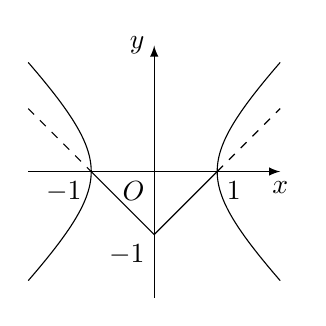
\begin{tikzpicture}[>=latex,scale = 0.8]
\draw [->] (-2,0) -- (2,0) node [below] {$x$};
\draw [->] (0,-2) -- (0,2) node [left] {$y$};
\draw (0,0) node [below left] {$O$};
\draw [domain = -{sqrt(3)}:{sqrt(3)},samples = 100] plot ({sqrt(\x*\x+1)},\x);
\draw [domain = -{sqrt(3)}:{sqrt(3)},samples = 100] plot ({-sqrt(\x*\x+1)},\x);
\draw (-1,0) node [below left] {$-1$} -- (0,-1) node [below left] {$-1$} -- (1,0) node [below right] {$1$};
\draw [dashed] (-2,1) -- (-1,0) (1,0) -- (2,1);
\end{tikzpicture}
\end{center}
\twoch{$(|x|-y-1)\cdot (1-x^2+y^2)=0$}{$\sqrt {|x|-y-1}\cdot (1-x^2+y^2)=0$}{$(|x|-y-1)\cdot \sqrt {1-x^2+y^2}=0$}{$\sqrt {|x|-y-1}\cdot \sqrt {1-x^2+y^2}=0$}
\item 在正方体$ABCD-A_1B_1C_1D_1$的八个顶点中任取两个点作直线, 与直线$A_1B$异面且夹角成$60^{\circ}$的直线的条数为\bracket{20}.
\fourch{$3$}{$4$}{$5$}{$6$}
\item 已知正方体$ABCD-A_1B_1C_1D_1$的棱长为$2$, 点$E$、$F$分别是所在棱$A_1B_1$、$AB$的中点, 点$O_1$是面$A_1B_1C_1D_1$的中心, 如图所示.
\begin{center}
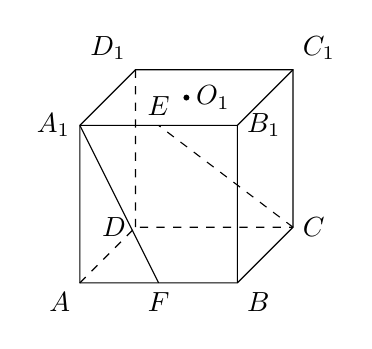
\begin{tikzpicture}[>=latex]
\draw (0,0) node [below left] {$A$} coordinate (A) --++ (2,0) node [below right] {$B$} coordinate (B) --++ (45:{2/2}) node [right] {$C$} coordinate (C)
--++ (0,2) node [above right] {$C_1$} coordinate (C1)
--++ (-2,0) node [above left] {$D_1$} coordinate (D1) --++ (225:{2/2}) node [left] {$A_1$} coordinate (A1) -- cycle;
\draw (A) ++ (2,2) node [right] {$B_1$} coordinate (B1) -- (B) (B1) --++ (45:{2/2}) (B1) --++ (-2,0);
\draw [dashed] (A) --++ (45:{2/2}) node [left] {$D$} coordinate (D) --++ (2,0) (D) --++ (0,2);
\draw (A1) -- ($(A)!0.5!(B)$) node [below] {$F$};
\draw [dashed] (C) -- ($(A1)!0.5!(B1)$) node [above] {$E$};
\filldraw ($(A1)!0.5!(C1)$) circle (0.03) node [right] {$O_1$};
\end{tikzpicture}
\end{center}
(1) 求三棱锥$O_1-FBC$的体积$V_{O_1-FBC}$;\\
(2) 求异面直线$A_1F$与$CE$所成角的大小.
\item 已知函数$f(x)=\dfrac a{2^x-1}+b$, 其中$a$、$b\in \mathbf{R}$.\\
(1) 当$a=6$, $b=0$时, 求满足$f(|x|)=2^x$的$x$的值;\\
(2) 若$f(x)$为奇函数且非偶函数, 求$a$与$b$的关系式.
\item 如图, 某大型厂区有三个值班室$A$、$B$、$C$, 值班室$A$在值班室$B$的正北方向$2$千米处, 值班室$C$在值班室$B$的正东方向$2\sqrt 3$千米处.
\begin{center}
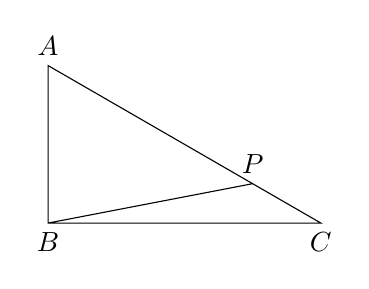
\begin{tikzpicture}[>=latex]
\draw (0,0) node [below] {$B$} coordinate (B);
\draw ({2*sqrt(3)},0) node [below] {$C$} coordinate (C);
\draw (0,2) node [above] {$A$} coordinate (A);
\draw ($(C)!0.25!(A)$) node [above] {$P$} coordinate (P);
\draw (A) -- (B) -- (C) -- cycle (B) -- (P);
\end{tikzpicture}
\end{center}
(1) 保安甲沿$CA$从值班室$C$出发行至点$P$处, 此时$PC=1$, 求$PB$的距离;\\
(2) 保安甲沿$CA$从值班室$C$出发前往值班室$A$, 保安乙沿$AB$从值班室$A$出发前往值班室$B$, 甲乙同时出发, 甲的速度为$1$千米/小时, 乙的速度为$2$千米/小时, 若甲乙两人通过对讲机联系, 对讲机在厂区的最大通话距离为$3$千米(含$3$千米), 试问有多长时间两人不能通话?
\item 已知椭圆$\Gamma:\dfrac{x^2}9+\dfrac{y^2}4=1$.\\
(1) 若抛物线$C$的焦点与$\Gamma$的焦点重合, 求$C$的标准方程;\\
(2) 若$\Gamma$的上顶点$A$、右焦点$F$及$x$轴上一点$M$构成直角三角形, 求点$M$的坐标;\\
(3) 若$O$为$\Gamma$的中心, $P$为$\Gamma$上一点(非$\Gamma$的顶点), 过$\Gamma$的左顶点$B$, 作$BQ\parallel OP$, $BQ$交$y$轴于点$Q$, 交$\Gamma$于点$N$, 求证: $\overrightarrow{BN}\cdot \overrightarrow{BQ}=2\overrightarrow{OP}^2$.
\item 给定整数$n$($n\ge 4$), 设集合$A=\{a_1,a_2,\cdots ,a_n\}$, $B=\{a_i+a_j|a_i,a_j\in A,\ 1\le i\le j\le n\}$.\\
(1) 若$A=\{-3,0,1,2\}$, 求集合$B$;\\
(2) 若$a_1,a_2,\cdots ,a_n$构成以$a_1$为首项, $d$($d>0$)为公差的等差数列, 求证: 集合$B$中的元素个数为$2n-1$;\\
(3) 若$a_1,a_2,\cdots ,a_n$构成以$3$为首项, $3$为公比的等比数列, 求集合$B$中元素的个数及所有元素之和.

%zmj5
\item 已知集合$A=\mathbf{N}^*$, $B=\{x||2x-1|<5\}$, 则$A\cap B=$\blank{50}. (用列举法表示)
\item 已知复数$z$满足$z\mathrm{i}=2+\mathrm{i}$($\mathrm{i}$为虚数单位), 则$z=$\blank{50}.
\item 若函数$f(x)=2^x+1$的图像与$g(x)$的图像关于直线$y=x$对称, 则$g(9)=$\blank{50}.
\item 若$\tan (\alpha +\dfrac{\pi }4)=-3$, 则$\tan \alpha =$\blank{50}.
\item 在$(1-2x)^6$的二项展开式中, $x^3$项的系数为\blank{50}. (用数字作答)
\item 如图, 已知正四棱柱$ABCD-A_1B_1C_1D_1$的底面边长为$2$, 高为$3$, 则异面直线$AA_1$与$BD_1$所成角的大小是\blank{50}.
\begin{center}
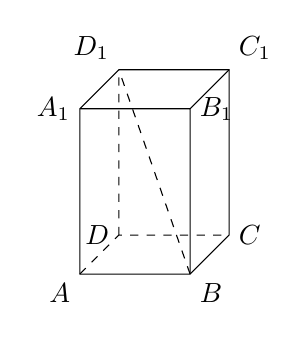
\begin{tikzpicture}[>=latex,scale = 0.7]
\draw (0,0) node [below left] {$A$} coordinate (A) --++ (2,0) node [below right] {$B$} coordinate (B) --++ (45:{2/2}) node [right] {$C$} coordinate (C)
--++ (0,3) node [above right] {$C_1$} coordinate (C1)
--++ (-2,0) node [above left] {$D_1$} coordinate (D1) --++ (225:{2/2}) node [left] {$A_1$} coordinate (A1) -- cycle;
\draw (A) ++ (2,3) node [right] {$B_1$} coordinate (B1) -- (B) (B1) --++ (45:{2/2}) (B1) --++ (-2,0);
\draw [dashed] (A) --++ (45:{2/2}) node [left] {$D$} coordinate (D) --++ (2,0) (D) --++ (0,3);
\draw [dashed] (B) -- (D1);
\end{tikzpicture}
\end{center}
\item 新冠病毒爆发初期, 全国支援武汉的活动中, 需要从$A$医院某科室的$6$名男医生(含一名主任医师)、$4$名女医生(含一名主任医师)中分别选派$3$名男医生和$2$名女医生, 要求至少有一名主任医师参加, 则不同的选派方案共有\blank{50}种. (用数字作答)
\item 设$k\in \{-2,-1,\dfrac 13,\dfrac 23,2\}$, 若对任意$x\in (-1,0)\cup (0,1)$, 都成立$x^k>|x|$, 则$k$取值的集合是\blank{50}.
\item 某校开设$9$门选修课程, 其中$A$, $B$, $C$三门课程由于上课时间相同, 至多选一门, 若规定每位学生选修$4$门, 则一共有\blank{50}种不同的选修方案.
\item 如图所示, 在平面直角坐标系$xOy$中, 动点$P$以每秒$\dfrac{\pi }2$的角速度从点$A$出发, 沿半径为$2$的上半圆逆时针移动到$B$, 再以每秒$\dfrac{\pi }3$的角速度从点$B$沿半径为1的下半圆逆时针移动到坐标原点$O$, 则上述过程中动点$P$的纵坐标$y$关于时间$t$的函数表达式为\blank{50}.
\begin{center}
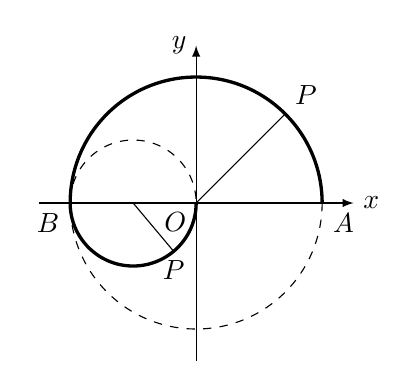
\begin{tikzpicture}[>=latex]
\draw [->] (-2,0) -- (2,0) node [right] {$x$};
\draw [->] (0,-2) -- (0,2) node [left] {$y$};
\draw (0,0) node [below left] {$O$};
\draw [very thick] (1.6,0) node [below right] {$A$} arc (0:180:1.6) node [below left] {$B$} arc (180:360:0.8);
\draw [dashed] (1.6,0) arc (0:-180:1.6) arc (-180:-360:0.8);
\draw (0,0) -- (45:1.6) node [above right] {$P$};
\draw (-0.8,0) --++ (-50:0.8) node [below] {$P$};
\end{tikzpicture}
\end{center}
\item 设$a>0$, $a\ne 1$, $M>0$, $N>0$, 我们可以证明对数的运算性质如下:\\
因为$a^{\log_aM+\log_aN}=a^{\log_aM}a^{\log_aN}=MN$, \textcircled{1}\\
所以$\log_a(MN)=\log_aM+\log_aN$.\\
我们将\textcircled{1}式称为证明的``关键步骤''. 则证明$\log_a(M^r)=r\log_aM$(其中$M>0$, $r\in \mathbf{R}$)的``关键步骤''为\blank{50}.
\item 已知函数$f(x)=|x+\dfrac 1x|$, 给出下列命题:\\
\textcircled{1} 存在实数a, 使得函数$y=f(x)+f(x-a)$为奇函数;\\
\textcircled{2} 对任意实数a, 均存在实数m, 使得函数$y=f(x)+f(x-a)$关于$x=m$对称;\\
\textcircled{3} 若对任意非零实数a, $f(x)+f(x-a)\ge k$都成立, 则实数$k$的取值范围为$(-\infty ,4]$;\\
\textcircled{4} 存在实数k, 使得函数$y=f(x)+f(x-a)-k$对任意非零实数a均存在6个零点.\\
其中的真命题是\blank{50}. (写出所有真命题的序号)
\item 若$a$为实数, 则``$a<1$''是``$\dfrac 1a>1$''的 \bracket{20}
\twoch{充分非必要条件}{必要非充分条件}{充要条件}{既非充分也非必要条件}
\item 若$\lg2=a$, $\lg3=b$, 则$\log_512$等于\bracket{20}
\fourch{$\dfrac{2a+b}{1+a}$}{$\dfrac{a^2b}{1+a}$}{$\dfrac{2a+b}{1-a}$}{$\dfrac{a^2b}{1-a}$}
\item 已知点$P$为双曲线$\dfrac{x^2}{a^2}-\dfrac{y^2}{b^2}=1$($a>0$, $b>0$)右支上一点, 点$F_1$, $F_2$分别为双曲线的左右焦点, 点$I$是$\triangle PF_1F_2$的内心(三角形内切圆的圆心), 若恒有$S_{\triangle IPF_1}-S_{\triangle IPF_2}=\dfrac{\sqrt 3}2S_{\triangle IF_1F_2}$, 则双曲线的渐近线方程是\bracket{20}.
\fourch{$y=\pm x$}{$y=\pm \dfrac{\sqrt 2}2x$}{$y=\pm \sqrt 3x$}{$y=\pm \dfrac{\sqrt 3}3x$}
\item 如图, 正四棱锥$P-ABCD$的底面边长和高均为$2$, $M$是侧棱$PC$的中点, 若过$AM$作该正四棱锥的截面, 分别交棱$PB$、$PD$于点$E$、$F$(可与端点重合), 则四棱锥$P-AEMF$的体积的取值范围是\bracket{20}.
\begin{center}
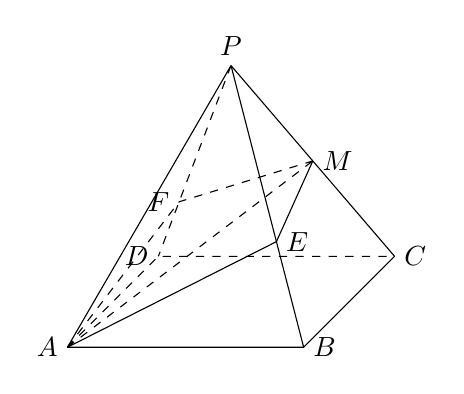
\begin{tikzpicture}[>=latex,scale = 1.5]
\draw (-1,0,1) node [left] {$A$} coordinate (A);
\draw (1,0,1) node [right] {$B$} coordinate (B);
\draw (1,0,-1) node [right] {$C$} coordinate (C);
\draw (-1,0,-1) node [left] {$D$} coordinate (D);
\draw (0,2,0) node [above] {$P$} coordinate (P);
\draw (P) -- (A) (P) -- (B) (P) -- (C) (A) -- (B) -- (C);
\draw [dashed] (P) -- (D) (A) -- (D) -- (C);
\draw ($(P)!0.5!(C)$) node [right] {$M$} coordinate (M);
\def\l{1.6}
\draw ($(P)!{1/\l}!(B)$) node [right] {$E$} coordinate (E);
\draw ($(P)!{1/(3-\l)}!(D)$) node [left] {$F$} coordinate (F);
\draw (A) -- (E) -- (M);
\draw [dashed] (A) -- (F) -- (M) (A) -- (M);
\end{tikzpicture}
\end{center}
\fourch{$[\dfrac 12,1]$}{$[\dfrac 12,\dfrac 43]$}{$[1,\dfrac 43]$}{$[\dfrac 89,1]$}
\item 如图, 在圆柱$OO_1$ 中, $AB$是圆柱的母线, $BC$是圆柱的底面$\odot O$的直径, $D$是底面圆周上异于$B$、$C$的点.
\begin{center}
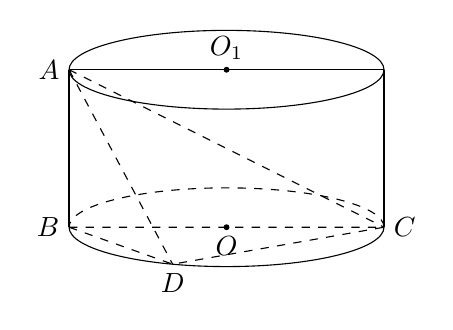
\begin{tikzpicture}[>=latex]
\draw (2,0) arc (0:-180:2 and 0.5);
\draw (2,2) arc (0:360:2 and 0.5);
\draw [dashed] (2,0) arc (0:180:2 and 0.5);
\draw (-2,2) node [left] {$A$} coordinate (A) -- (-2,0) node [left] {$B$} coordinate (B);
\draw (2,2) -- (2,0) node [right] {$C$} coordinate (C);
\draw ({2*cos(-110)},{0.5*sin(-110)}) node [below] {$D$} coordinate (D);
\draw [dashed] (B) -- (D) -- (C) (A) -- (C) (B) -- (C) (A) -- (D);
\draw (-2,2) -- (2,2);
\filldraw (0,0) circle (0.03) node [below] {$O$} coordinate (O);
\filldraw (0,2) circle (0.03) node [above] {$O_1$} coordinate (O1);
\end{tikzpicture}
\end{center}
(1) 求证:  $CD\perp$平面$ABD$;\\
(2) 若$BD=2$, $CD=4$, $AC=6$, 求圆柱$OO_1$的侧面积.
\item 已知函数$f(x)=2\sqrt 2\sin \dfrac x2\cos \dfrac x2+2\sqrt 2\cos ^2\dfrac x2-\sqrt 2$.\\
(1) 求函数$f(x)$在区间$[0,\pi]$上的值域;\\
(2) 若方程$f(\omega x)=\sqrt 3(\omega >0)$在区间$[0,\pi]$上至少有两个不同的解, 求$\omega$的取值范围.
\item 大数据时代对于数据分析能力的要求越来越高, 数据拟合是一种把现有数据通过数学方法来代入某种算式的表示方式. 比如$A_i(a_i,b_i)$($i=1,2,3,\cdots,n$)是平面直角坐标系上的一系列点, 其中$n$是不小于$2$的正整数, 用函数$y=f(x)$来拟合该组数据, 尽可能使得函数图像与点列$(a_i,b_i)$比较接近. 其中一种衡量接近程度的指标是函数的拟合误差, 拟合误差越小越好, 定义函数$y=f(x)$的拟合误差为:
$\Delta (f(x))=\dfrac 1n[(f(a_1)-b_1)^2+(f(a_2)-b_2)^2+\cdots +(f(a_n)-b_n)^2]$.\\
已知在平面直角坐标系上, 有$5$个点的坐标数据如下表所示:
\begin{center}
\begin{tabular}{|c|c|c|c|c|c|}
\hline
$x$  & $1$  & $2$  & $3$  & $4$  & $5$ \\ \hline
$y$  & $2.2$  & $1$  & $2$  & $4.6$  & $7$ \\ \hline
\end{tabular}
\end{center}
(1)若用函数$f_1(x)=x^2-4x+5$来拟合上述表格中的数据, 求$\Delta (f_1(x))$;\\
(2)若用函数$f_2(x)=2^{|x-2|}+m$来拟合上述表格中的数据.\\
\textcircled{1} 求该函数的拟合误差$\Delta (f_2(x))$的最小值, 并求出此时的函数解析式$y=f_2(x)$;\\
\textcircled{2} 指出用$f_1(x),f_2(x)$(指\textcircled{1}中使$\Delta(f_2(x))$最小的函数)中的哪一个函数来拟合上述表格中的数据更好?
\item 对于函数$y=f(x)$, 若函数$F(x)=f(x+1)-f(x)$是增函数, 则称函数$y=f(x)$具有性质$A$.\\
(1) 若$f(x)=x^2+2^x$, 求$F(x)$的解析式, 并判断$f(x)$是否具有性质$A$;\\
(2) 判断命题``减函数不具有性质$A$''是否真命题, 并说明理由;\\
(3) 若函数$f(x)=kx^2+x^3(x\ge 0)$具有性质$A$, 求实数$k$的取值范围, 并讨论此时函数$g(x)=f(\sin x)-\sin x$在区间$[0,\pi]$上零点的个数.
\item 现定义: 设$a$是非零实常数, 若对于任意的$x\in D$, 都有$f(a-x)=f(a+x)$, 则称函数$y=f(x)$为``关于$a$的偶型函数''.\\
(1) 请以三角函数为例, 写出一个``关于$2$的偶型函数''的解析式, 并给予证明;\\
(2) 设定义域为$\mathbf{R}$的``关于$a$的偶型函数''$y=f(x)$在区间$(-\infty ,a)$上单调递增, 求证: $y=f(x)$在区间$(a,+\infty)$上单调递减;\\
(3) 设定义域为$\mathbf{R}$的``关于$\dfrac 12$的偶型函数''$y=f(x)$是奇函数. 若$n\in \mathbf{N}^*$, 请猜测$f(n)$的值, 并用数学归纳法证明你的结论.

%zmj6
\item 若集合$A=\{x|1\le x\}$, $B=\{-1,1,2,3\}$, 则$A\cap B=$\blank{50}.
\item 已知复数$z$满足$z\cdot (1-\mathrm{i})=1+3\mathrm{i}$($\mathrm{i}$为虚数单位), 则$|z|=$\blank{50}.
\item 若$\sin \alpha =\dfrac 13$, 则$\sin (\dfrac \pi 2-2\alpha)=$\blank{50}.
\item 已知圆锥的母线$l=2$, 母线与旋转轴的夹角$\alpha =30^{\circ}$, 则圆锥的侧面积为\blank{50}.
\item 已知函数$f(x)$图像与函数$g(x)=2^x$的图像关于$y=x$对称, 则$f(4)=$\blank{50}.
\item 若关于$x$、$y$的方程组$\begin{cases} 2x+3y=1 \\ ax-y=2 \end{cases}$无解, 则实数$a=$\blank{50}.
\item 在$\triangle ABC$中, 角$A$、$B$、$C$所对的边分别为$a$、$b$、$c$, 且$\begin{vmatrix}   \sqrt 3b+2c & 2a  \\\cos B & 1  \end{vmatrix}=0$, 则角$A=$\blank{50}.
\item 已知$A,B$分别是函数$f(x)=2\sin \omega x$($\omega >0$)在$y$轴右侧图像上的第一个最高点和第一个最低点, 且$\angle AOB=\dfrac\pi 2$, 则该函数的最小正周期是\blank{50}.
\item 疫情期间家长会, 我校要从$5$名男生, $3$名女生中选派$4$名志愿者担任家长入校测量体温、查看行程码、健康码、登记信息四项不同的工作, 若其中女生不能从事测量体温, 则不同的选派方案共有\blank{50}种.
\item 正方形$ABCD$的边长为$4$, $O$是正方形$ABCD$的中心, 过中心$O$的直线$l$与边$AB$交于点$M$, 与边$CD$交于点$N$, $P$为平面上一点, 满足: 存在$\lambda\in \mathbf{R}$, 使得$2\overrightarrow{OP}=\lambda \overrightarrow{OB}+(1-\lambda)\overrightarrow{OC}$, 则$\overrightarrow{PM}\cdot \overrightarrow{PN}$的最小值为\blank{50}.
\item 若函数$f(x)=\begin{cases}|\lg (x-1)|, & x>1,  \\ \sin x, &  x<0, \end{cases}$ 则$y=f(x)$图像上关于原点$O$对称的点共有\blank{50}对.
\item 已知函数$y=f(x)$, 对任意$x\in \mathbf{R}$, 都有$f(x+2)\cdot f(x)=k$($k$为常数), 且当$x\in [0,2]$时, $f(x)=x^2+1$, 则$f(2022)=$\blank{50}.
\item 已知$l$是平面$\alpha$的一条斜线, 直线$m\subseteq \alpha$, 则\bracket{20}.
\twoch{存在唯一的一条直线$m$, 使得$l\perp m$}{存在无限多条直线$m$, 使得$l\perp m$}{存在唯一的一条直线$m$, 使得$l \parallel m$}{存在无限多条直线$m$, 使得$l \parallel m$}
\item 在正方体$ABCD-A_1B_1C_1D_1$ 中, 下列四个结论中错误的是\bracket{20}.
\begin{center}
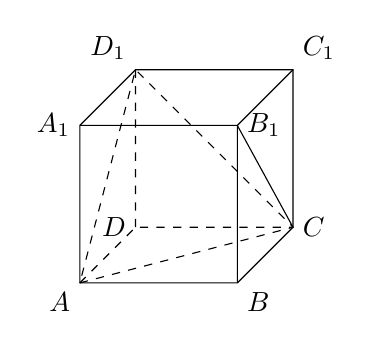
\begin{tikzpicture}[>=latex]
\draw (0,0) node [below left] {$A$} coordinate (A) --++ (2,0) node [below right] {$B$} coordinate (B) --++ (45:{2/2}) node [right] {$C$} coordinate (C)
--++ (0,2) node [above right] {$C_1$} coordinate (C1)
--++ (-2,0) node [above left] {$D_1$} coordinate (D1) --++ (225:{2/2}) node [left] {$A_1$} coordinate (A1) -- cycle;
\draw (A) ++ (2,2) node [right] {$B_1$} coordinate (B1) -- (B) (B1) --++ (45:{2/2}) (B1) --++ (-2,0);
\draw [dashed] (A) --++ (45:{2/2}) node [left] {$D$} coordinate (D) --++ (2,0) (D) --++ (0,2);
\draw (C) -- (B1);
\draw [dashed] (A) -- (C) -- (D1) -- cycle;
\end{tikzpicture}
\end{center}
\twoch{直线$B_1C$与直线$AC$所成的角为$60^\circ$}{直线$B_1C$与平面$AD_1C$所成的角为$60^\circ$}{直线$B_1C$与直线$AD_1$所成的角为$90^\circ$}{直线$B_1C$与直线$AB$所成的角为$90^\circ$}
\item 若$a<b$, 则下列不等式恒成立的是\bracket{20}.
\fourch{$|a|<|b|$}{$-a>b$}{$a^2>b^2$}{$\sqrt[3]a<\sqrt[3]b$}
\item 记$S_n$为数列$\{a_n\}$的前$n$项和, 已知点$(n,a_n)$在直线$y=10-2x$上, 若有且只有四个正整数$n$满足$S_n\ge k$, 则实数$k$的取值范围是\bracket{20}.
\fourch{$(8,14]$}{$(14,18]$}{$(18,20]$}{$(18,\dfrac{81}4]$}
\item 在直三棱柱$ABC-A_1B_1C_1$中, $\angle ABC=90^\circ$, $AB=BC=1$, $BB_1=2$.
\begin{center}
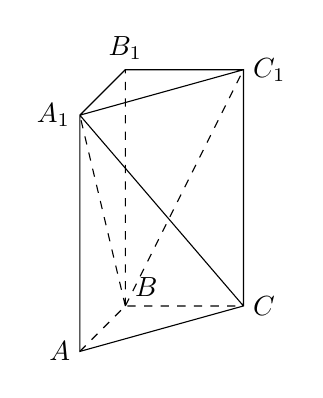
\begin{tikzpicture}[>=latex,scale = 1.5]
\draw (0,0,0) node [above right] {$B$} coordinate (B);
\draw (1,0,0) node [right] {$C$} coordinate (C);
\draw (0,0,1) node [left] {$A$} coordinate (A);
\draw (A) ++ (0,2,0) node [left] {$A_1$} coordinate (A1);
\draw (B) ++ (0,2,0) node [above] {$B_1$} coordinate (B1);
\draw (C) ++ (0,2,0) node [right] {$C_1$} coordinate (C1);
\draw (A) -- (C) -- (C1) -- (A1) -- cycle (A1) -- (B1) -- (C1) (A1) -- (C);
\draw [dashed] (A) -- (B) -- (C) (B) -- (B1) (B) -- (A1) (B) -- (C1);
\end{tikzpicture}
\end{center}
(1) 求异面直线$B_1C_1$与$A_1C$所成角的大小;\\
(2) 求点$C_1$与平面$A_1BC$的距离.
\item 已知函数$f(x)=\sqrt 3\sin x\cos x-\sin ^2x+2$.\\
(1) 求$f(x)$的最小正周期和值域;\\
(2) 若对任意的$x\in \mathbf{R}$, $f^2(x)-k\cdot f(x)+1\le 0$恒成立, 求实数$k$的取值范围.
\item 如图, 上海天马山上的``护珠塔''因其倾斜度超过意大利的比萨斜塔而号称``世界第一斜塔'', 兴趣小组同学实施如下方案来测量塔的倾斜度和塔高, 如图, 记$O$点为塔基、$P$点为塔尖、点$P$在地面上的射影为点$H$, 在塔身$OP$射影所在直线上选点$A$, 使仰角$\angle HAP=45^{^\circ }$, 过$O$点与$OA$成$120^{^\circ }$的地面上选$B$点, 使仰角$\angle HBP=45^\circ$(点$A$、$B$、$O$都在同一水平面上), 此时测得$\angle OAB=27^\circ$, $A$与$B$之间距离为$33.6$米, 试求:
\begin{center}
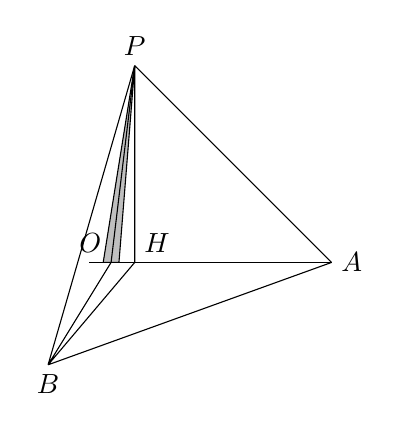
\begin{tikzpicture}[>=latex]
\draw (0,0) node [above left] {$O$} coordinate (O);
\draw (O) ++ (0.1,0) coordinate (O1);
\draw (O) ++ (-0.1,0) coordinate (O2);
\draw (0.3,0) node [above right] {$H$} coordinate (H);
\draw (2.8,0) node [right] {$A$} coordinate (A);
\draw (0.3,2.5) node [above] {$P$} coordinate (P);
\draw (-0.8,-1.3) node [below] {$B$} coordinate (B);
\filldraw [fill = gray!50, draw = black] (P) -- (O1) -- (O2) -- cycle; 
\draw (B) -- (O)  (B) -- (H) (B) -- (A) (O) -- (P) (H) -- (P) (A) -- (P) (B) -- (P);
\draw (A) -- ($(A)!1.1!(O)$);
\end{tikzpicture}
\end{center}
(1) 塔高(即线段$PH$的长, 精确到$0.1$米);\\
(2) 塔的倾斜度(即$\angle OPH$的大小, 精确到$0.1^\circ$).
\item 如图, 在长方体$ABCD-A_1B_1C_1D_1$中, $AD=AA_1=1$, $AB\text=2$, 点$E$在棱$AB$上移动.
\begin{center}
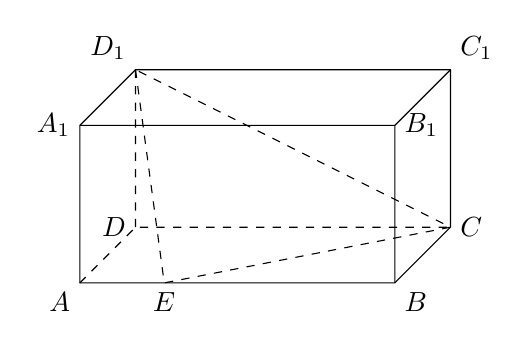
\begin{tikzpicture}[>=latex,scale = 2]
\draw (0,0) node [below left] {$A$} coordinate (A) --++ (2,0) node [below right] {$B$} coordinate (B) --++ (45:{1/2}) node [right] {$C$} coordinate (C)
--++ (0,1) node [above right] {$C_1$} coordinate (C1)
--++ (-2,0) node [above left] {$D_1$} coordinate (D1) --++ (225:{1/2}) node [left] {$A_1$} coordinate (A1) -- cycle;
\draw (A) ++ (2,1) node [right] {$B_1$} coordinate (B1) -- (B) (B1) --++ (45:{1/2}) (B1) --++ (-2,0);
\draw [dashed] (A) --++ (45:{1/2}) node [left] {$D$} coordinate (D) --++ (2,0) (D) --++ (0,1);
\draw ($(A)!{2-sqrt(3)}!(B)$) node [below] {$E$} coordinate (E);
\draw [dashed] (D1) -- (E) -- (C) -- cycle;
\end{tikzpicture}
\end{center}
(1) 证明: $D_1E\perp A_1D$;\\
(2) 当$E$为$AB$的中点时, 求直线$A_1E$与面$ACD_1$所成角的正弦值;\\
(3) 棱$AB$上是否存在点$E$, 使得二面角$D_1-EC-D$的大小为$\dfrac{\pi }4$, 若存在求出$AE$的长; 若不存在说明理由.
\item 设$f(x)=\dfrac{-2^x+a}{2^{x+1}+b}$, $a,b$为实常数.\\
(1) 当$a=b=1$时, 证明: $f(x)$不是奇函数;\\
(2) 若$f(x)$是奇函数, 求$a$与$b$的值.

%zmj9
\item 已知集合$A=\{1,3,5,6,7\}$, $B=\{2,4,5,6,8\}$, 则$A\cap B=$\blank{50}.
\item 不等式$|3x-2|<1$的解集是\blank{50}.
\item 已知$(2x^2-\dfrac 1x)^n$($n\in \mathbf{N}^*)$的展开式中各项的二项式系数之和为$128$, 则其展开式中含$\dfrac 1x$项的系数是\blank{50}.(结果用数值表示)
\item 已知函数$f(x)$是以$2$为周期的偶函数, 当$0\le x\le 1$时, $f(x)=\lg (x+1)$, 令函数$g(x)=f(x)(x\in [1,2])$, 则$g(x)$的反函数为\blank{50}.
\item 若$x>0$, $y>0$, 且$4x+y=xy$, 则$x+y-m\ge 0$恒成立的实数$m$的取值范围是\blank{50}.
\item 已知函数$f(x)=A\sin (\omega x+\varphi)$($\omega >0$, $0<\varphi <\dfrac{\pi }2$)的部分图像如图所示, 则函数$f(x)$的解析式为\blank{50}.
\begin{center}
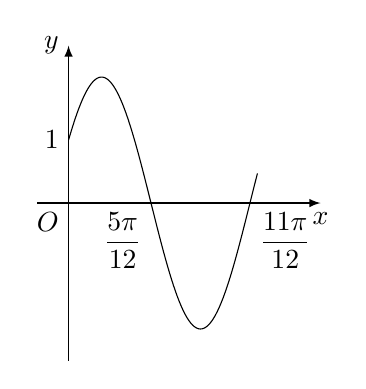
\begin{tikzpicture}[>=latex,scale = 0.8]
\draw [->] (-0.5,0) -- (4,0) node [below] {$x$};
\draw [->] (0,-2.5) -- (0,2.5) node [left] {$y$};
\draw (0,0) node [below left] {$O$};
\draw [domain = 0:3,samples = 100] plot (\x,{2*sin(2*\x/pi*180+30)});
\draw (0,1) node [left] {$1$};
\draw ({5*pi/12},0) node [below left] {$\dfrac{5\pi}{12}$};
\draw ({11*pi/12},0) node [below right] {$\dfrac{11\pi}{12}$};
\end{tikzpicture}
\end{center}
\item 在$120^\circ$的二面角内放置一个半径为$6$的小球, 它与二面角的两个半平面相切于$A$、$B$两点, 则这两个点在球面上的距离是\blank{50}.
\item 设函数$f(x)=\lg (1+|x|)-\dfrac 1{1+x^2}$, 则使得$f(2x)<f(3x-2)$成立的$x$的取值范围是\blank{50}.
\item 若偶函数$y=f(x)$($x\in \mathbf{R}$)满足$f(x+2)=f(x-2)$, 当$x\in [-2,0]$时, $f(x)=(\dfrac 12)^x-1$, 若$g(x)=f(x)-\log_a(x+2)$($a>1$)在区间$(-2,6]$上恰有$3$个不同的零点, 则实数$a$的取值范是\blank{50}
\item 已知函数$f(x)=x^2-a|x|+\dfrac 1{x^2+1}+a$有且只有一个零点, 若方程$f(x)=k$无解, 则实数$k$的取值范围为\blank{50}.
\item 设函数$f(x)$的定义域是$(0,1)$, 满足: \textcircled{1} 对任意的$x\in (0,1)$, $f(x)>0$; \textcircled{2} 对任意的$x_1$、$x_2\in (0,1)$, 都有$\dfrac{f(x_1)}{f(x_2)}+\dfrac{f(1-x_1)}{f(1-x_2)}\le 2$; \textcircled{3} $f(\dfrac 12)=2$. 则函数$g(x)=xf(x)+\dfrac 1x$的最小值为\blank{50}.
\item 用$M_I$表示函数$y=\sin x$在闭区间$I$上的最大值, 若正数$a$满足$M_{[0,a]}\ge 2M_{[a,2a]}$, 则$a$的最大值为\blank{50}.
\item 魏晋时期数学家刘徽在他的著作《九章算术注》中, 称一个正方体内两个互相垂直的内切圆柱所围成的几何体为``牟合方盖''. 刘徽通过计算得知正方体的内切球的体积与``牟合方盖''的体积之比应为$\pi:4$. 若正方体的棱长为$2$, 则``牟合方盖''的体积为\bracket{20}.
\fourch{$16$}{$16\sqrt 3$}{$\dfrac{16}3$}{$\dfrac{128}3$}
\item 若$f(x)$是$\mathbf{R}$上的奇函数, 且$f(x)$在$[0,+\infty)$上单调递增, 则下列结论:\\
\textcircled{1} $y=|f(x)|$是偶函数;\\
\textcircled{2} 对任意$x\in \mathbf{R}$都有$f(-x)+|f(x)|=0$;\\
\textcircled{3} $y=f(x)f(-x)$在$(-\infty ,0]$上单调递增;\\
\textcircled{4} 反函数$y=f^{-1}(x)$存在且在$(-\infty ,0]$上单调递增.\\
其中正确结论的个数为\bracket{20}.
\fourch{$1$}{$2$}{$3$}{$4$}
\item 函数$f(x)$的定义域为$D$, 若$f(x)$存在反函数, 且$f(x)$的反函数就是它本身, 则称$f(x)$为自反函数, 有下列四个命题:\\
\textcircled{1} 函数$f(x)=-\dfrac x{x+1}$是自反函数;\\
\textcircled{2} 若$f(x)$为自反函数, 则对任意的$x\in D$, 成立$f(f(x))=x$;
\textcircled{3} 若函数$f(x)=\sqrt {1-x^2}$($a\le x\le b$)为自反函数, 则$b-a$的最大值为$1$;\\
\textcircled{4} 若$f(x)$是定义在$\mathbf{R}$上的自反函数, 则方程$f(x)=x$有解;\\
其中正确命题的序号为\bracket{20}.
\fourch{\textcircled{1}\textcircled{2}\textcircled{3}}{\textcircled{1}\textcircled{2}\textcircled{4}}{\textcircled{2}\textcircled{3}\textcircled{4}}{\textcircled{1}\textcircled{2}\textcircled{3}\textcircled{4}}
\item 设函数$f(x)$的定义域为$\mathbf{R}$, 满足$f(x+1)=2f(x)$, 且当$x\in (0,1]$时, $f(x)=x(x-1)$.
若对任意$x\in (-\infty ,m]$, 都有$f(x)\ge -\dfrac 89$, 则$m$的取值范围是\bracket{20}.
\fourch{$(-\infty ,\dfrac 94]$}{$(-\infty ,\dfrac 73]$}{$(-\infty ,\dfrac 52]$}{$(-\infty ,\dfrac 83]$}
\item 如图, 已知正方体$ABCD-A'B'C'D'$的棱长为$1$.
\begin{center}
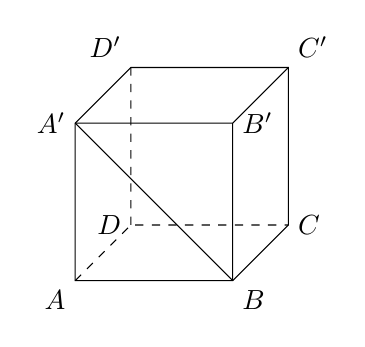
\begin{tikzpicture}[>=latex]
\draw (0,0) node [below left] {$A$} coordinate (A) --++ (2,0) node [below right] {$B$} coordinate (B) --++ (45:{2/2}) node [right] {$C$} coordinate (C)
--++ (0,2) node [above right] {$C'$} coordinate (C1)
--++ (-2,0) node [above left] {$D'$} coordinate (D1) --++ (225:{2/2}) node [left] {$A'$} coordinate (A1) -- cycle;
\draw (A) ++ (2,2) node [right] {$B'$} coordinate (B1) -- (B) (B1) --++ (45:{2/2}) (B1) --++ (-2,0);
\draw [dashed] (A) --++ (45:{2/2}) node [left] {$D$} coordinate (D) --++ (2,0) (D) --++ (0,2);
\draw (A1) -- (B);
\end{tikzpicture}
\end{center}
(1) 正方体$ABCD-A'B'C'D'$中哪些棱所在的直线与直线$A'B$是异面直线?\\
(2) 若$M,N$分别是$A'B,BC'$的中点, 求异面直线$MN$与$BC$所成角的大小.
\item 已知函数$f(x)=\dfrac{ax-2}{x+2}$其中$a\in \mathbf{R}$.\\
(1) 解关于$x$的不等式$f(x)\le -1$;\\
(2) 求$a$的取值范围, 使$f(x)$在区间$(0,+\infty)$上是单调减函数.
\item 我国的``洋垃圾禁止入境''政策已实施一年多. 某沿海地区的海岸线为一段圆弧$\frown{AB}$, 对应的圆心角$\angle AOB=\dfrac\pi 3$. 该地区为打击洋垃圾走私, 在海岸线外侧$20$海里内的海域$ABCD$对不明船只进行识别查证(如图: 其中海域与陆地近似看作在同一平面内).在圆弧的两端点$A,B$分别建有监测站, $A$与$B$之间的直线距离为$100$海里.
\begin{center}
\begin{tikzpicture}[>=latex,scale = 1.3]
\draw (0,0) node [below] {$O$} coordinate (O);
\draw (50:2) node [right] {$B$} coordinate (B);
\draw (50:2.4) node [right] {$C$} coordinate (C);
\draw (110:2) node [left] {$A$} coordinate (A);
\draw (110:2.4) node [left] {$D$} coordinate (D);
\draw (B) arc (50:110:2) -- (D) arc (110:50:2.4) -- cycle;
\draw [dashed] (O) -- (A) (O) -- (B);
\draw (80:1.33) node {\rotatebox{-10}{陆地}};
\draw (80:2.2) node {\rotatebox{-10}{海域}};
\end{tikzpicture}
\end{center}
(1) 求海域$ABCD$的面积;\\
(2) 现海上$P$点处有一艘不明船只, 在$A$点测得其距$A$点$40$海里, 在$B$点测得其距$B$点$20\sqrt {19}$海里. 判断这艘不明船只是否进入了海域$ABCD$? 请说明理由.
\item 已知函数$f(x)$, 若存在非零常数$k$, 对于任意实数$x$, 都有$f(x+k)+f(x)=x$成立, 则称函数$f(x)$是``$M_k$类函数''.\\
(1) 若函数$f(x)=ax+b$是``$M_1$类函数'', 求实数$a$、$b$的值;\\
(2) 若函数$g(x)$是``$M_2$类函数'', 且当$x\in [0,2]$时, $g(x)=x(2-x)$, 求函数$g(x)$在$x\in [2,6]$时的最大值和最小值;\\
(3) 已知函数$f(x)$是``$M_k$类函数'', 是否存在一次函数$h(x)=Ax+B$(常数$A$、$B\in \mathbf{R}$, $A\ne 0$), 使得函数$F(x)=f(x)+h(x)$是周期函数, 说明理由.
\item 设$n$为正整数, 集合$A=\{\alpha|\alpha =(t_1,t_2,\cdots ,t_n),\ t_k\in \{0,1\}, \ k=1,2,\cdots,n\}$, 对于集合$A$中的任意元素$\alpha =(x_1,x_2,\cdots ,x_n)$和$\beta =(y_1,y_2,\cdots ,y_n)$, 记
$M(\alpha ,\beta)=\dfrac 12[(x_1+y_1-|x_1-y_1|)+(x_2+y_2-|x_2-y_2|)+\cdots +(x_n+y_n-|x_n-y_n|)]$.\\
(1) 当$n=3$时, 若$\alpha =(1,1,0)$, $\beta =(0,1,1)$, 求$M(\alpha ,\alpha)$和$M(\alpha ,\beta)$的值;\\
(2) 当$n=4$时, 设$B$是$A$的子集, 且满足: 对于$B$中的任意元素$\alpha$、$\beta$, 当$\alpha$、$\beta$相同时, $M(\alpha ,\beta)$是奇数; 当$\alpha$、$\beta$不同时, $M(\alpha ,\beta)$是偶数. 求集合$B$中元素个数的最大值;\\
(3) 给定不小于$2$的$n$, 设$B$是$A$的子集, 且满足: 对于$B$中的任意两个不同的元素$\alpha$、$\beta$, $M(\alpha ,\beta)=0$, 写出一个集合$B$, 使其元素个数最多, 并说明理由.

%zmj10
\item 已知集合$A=(-\infty ,-3)$, $B=(-4,+\infty)$, 则$A\cap B=$\blank{50}.
\item 行列式$\begin{vmatrix}   \sin \alpha &  \sin \alpha -\cos \alpha   \\\cos \alpha  & \sin \alpha +\cos \alpha   \end{vmatrix}$的值等于\blank{50}.
\item 已知复数$z$满足$\dfrac 1{z-1}=\mathrm{i}$($\mathrm{i}$为虚数单位), 则$z=$\blank{50}.
\item 函数$f(x)=\log_2(2x+4)$的反函数为$f^{-1}(x)$, 则$f^{-1}(4)=$\blank{50}.
\item 从甲、乙、丙、丁$4$名同学中随机选$2$名同学参加志愿者服务, 则甲、乙两人都没有被选到的概率为\blank{50}(用数字作答).
\item 已知二项式$(2x+\dfrac 1x)^6$, 则其展开式中的常数项为\blank{50}.
\item 计算: $\displaystyle\lim_{n\to \infty} \dfrac{|4n-23|}{2n}=$\blank{50}.
\item 已知圆锥的底面半径为$1$, 高为$\sqrt 3$, 则该圆锥的侧面展开图的圆心角$\theta$的大小为\blank{50}.
\item 已知$\alpha \in (0,\pi)$, 且有$1-2\sin 2\alpha =\cos 2\alpha$, 则$\cos \alpha =$\blank{50}.
\item 设$F_1,F_2$分别是双曲线$\dfrac{x^2}{a^2}-\dfrac{y^2}{b^2}=1$($a>0$, $b>0$)的左、右焦点, 点$P$在双曲线右支上且满足$|PF_2|=|F_1F_2|$, 双曲线的渐近线方程为$4x\pm 3y=0$, 则$\cos \angle PF_1F_2=$\blank{50}.
\item 若$a,b$分别是正数$p$, $q$的算术平均数和几何平均数, 且$a,b,-2$ 这三个数可适当排序后成等差数列, 也可适当排序后成等比数列, 则$p+q+pq$的值形成的集合是\blank{50}.
\item 设$f(x)=x^2+2a\cdot x+b\cdot 2^x$, 其中$a,b\in \mathbf{N}$, $x\in \mathbf{R}$, 如果函数$y=f(x)$与函数$y=f(f(x))$都有零点且它们的零点完全相同, 则有序数对$(a,b)$为\blank{50}.
\item 直线$x+3y-1=0$的一个法向量可以是\bracket{20}.
\fourch{$(3,-1)$}{$(3,1)$}{$(1,3)$}{$(-1,3)$}
\item 在$\triangle ABC$中, 若$\overrightarrow{AB}\cdot \overrightarrow{BC}+\overrightarrow{AB}^2=0$, 则$\triangle ABC$的形状一定是\bracket{20}.
\fourch{等边三角形}{直角三角形}{等腰三角形}{等腰直角三角形}
\item 已知函数$f(x)=A\sin (\omega x+\phi)$($A>0$, $\omega >0$)的图像与直线$y=b$($0<b<A$)的三个相邻交点的横坐标依次是$1,2,4$, 下列区间是函数$f(x)$单调递增区间的是\bracket{20}.
\fourch{$[0,3]$}{$[\dfrac 32,3]$}{$[3,6]$}{$[3,\dfrac 92]$}
\item 下列结论中错误的是\bracket{20}.
\onech{存在实数$x$、$y$满足$\begin{cases}|x|\le 1, \\|x+y|\le 1, \end{cases}$ 并使得$4(x+1)(y+1)>9$成立}{存在实数$x$、$y$满足$\begin{cases}|x|\le 1, \\|x+y|\le 1, \end{cases}$ 并使得$4(x+1)(y+1)>7$成立}{满足$\begin{cases}|x|\le 1, \\|x+y|\le 1, \end{cases}$ 且使得$4(x+1)(y+1)=-9$的实数$x$、$y$不存在}{满足$\begin{cases}|x|\le 1, \\|x+y|\le 1, \end{cases}$ 且使得$4(x+1)(y+1)<-9$的实数$x$、$y$不存在}
\item 如图在三棱锥$P-ABC$中, 棱$AB$、$AC$、$AP$两两垂直, $AB=AC=AP=3$, 点$M$在$AP$上, 且$AM=1$.
\begin{center}
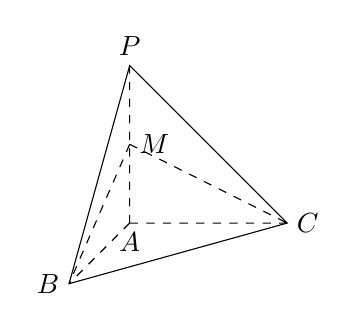
\begin{tikzpicture}[>=latex]
\draw (0,0,0) node [below] {$A$} coordinate (A);
\draw (2,0,0) node [right] {$C$} coordinate (C);
\draw (0,0,2) node [left] {$B$} coordinate (B);
\draw (0,2,0) node [above] {$P$} coordinate (P);
\draw ($(A)!0.5!(P)$) node [right] {$M$} coordinate (M);
\draw (P) -- (B) -- (C) -- cycle;
\draw [dashed] (A) -- (B) (A) -- (C) (A) -- (P) (M) -- (B) (M) -- (C);
\end{tikzpicture}
\end{center}
(1) 求异面直线$BM$和$PC$所成的角的大小;\\
(2) 求三棱锥$P-BMC$的体积.
\item 已知函数$f(x)=\sin x\cos (\dfrac{\pi }2+x)+\sqrt 3\sin x\cos x$.\\
(1) 求函数$f(x)$的最小正周期及对称中心;\\
(2) 若$f(x)=a$在区间$[0,\dfrac{\pi }2]$上有两个解$x_1,x_2$, 求$a$的取值范围及$x_1+x_2$的值.
\item 某企业接到生产$3000$台某产品的甲、乙、丙$3$种部件的订单, 每台产品需要这$3$种部件的数量分别为$2, 2, 1$(单位: 件). 已知每个工人每天可生产甲部件$6$件, 或乙部件$3$件, 或丙部件$2$件. 该企业计划安排$200$名工人分成三组分别生产这$3$种部件, 生产乙部件的人数与生产甲部件的人数成正比例, 比例系数为$k$($k\ge 2$为正整数).\\
(1) 设生产甲部件的人数为$x$, 分别写出完成甲、乙、丙$3$种部件生产需要的时间;\\
(2) 假设这$3$种部件的生产同时开工, 试确定正整数$k$的值, 使完成订单任务的时间最短, 并给出时间最短时具体的人数分组方案.
\item 已知$F_1$、$F_2$分别为椭圆$\Gamma :\dfrac{x^2}4+y^2=1$的左、右焦点, $M$为$\Gamma$上的一点.
\begin{center}
\begin{tikzpicture}[>=latex]
\def\r{0.75}
\draw [->] (-2.5,0) -- (2.5,0) node [below] {$x$};
\draw [->] (0,-1.5) -- (0,2) node [left] {$y$};
\draw (0,0) node [below left] {$O$};
\draw [name path = ellipse] (0,0) ellipse (2 and 1);
\filldraw ({2*cos(75)},{sin(75)}) circle (0.03) node [above] {$M$} coordinate (M);
\draw (M) circle (\r);
\draw [name path = tangent1] ($(O)!2.2!{-asin(\r/sqrt(4*pow(cos(75),2)+pow(sin(75),2)))}:(M)$) -- (O);
\draw [name path = tangent2] ($(O)!1.5!{asin(\r/sqrt(4*pow(cos(75),2)+pow(sin(75),2)))}:(M)$) -- (O);
\draw [name intersections = {of = tangent1 and ellipse, by = P}];
\draw [name intersections = {of = tangent2 and ellipse, by = Q}];
\draw (P) node [above] {$P$};
\draw (Q) node [below left] {$Q$};
\end{tikzpicture}
\end{center}
(1) 若点$M$的坐标为$(1,m)$($m>0$), 求$\triangle F_1MF_2$的面积;\\
(2) 若点$M$的坐标为$(0,1)$, 且直线$y=kx-\dfrac 35$($k\in \mathbf{R}$)与$\Gamma$交于两不同点$A$、$B$, 求证: $\overrightarrow{MA}\cdot \overrightarrow{MB}$为定值, 并求出该定值;\\
(3)如图, 设点$M$的坐标为$(s,t)$, 过坐标原点$O$作圆$M:(x-s)^2+(y-t)^2=r^2$(其中$r$为定值, $0<r<1$, 且$|s|\ne r$)的两条切线, 分别交$\Gamma$于点$P$、$Q$, 直线$OP$、$OQ$的斜率分别记为$k_1$、$k_2$, 如果$k_1k_2$为定值, 试问: 是否存在锐角$\theta$, 使得$2|OP|\cdot|OQ|=5\cdot \sec \theta$? 若存在, 试求出$\theta$的一个值; 若不存在, 请说明理由.
\item 设$x$是实数, $n$是整数, 若$|x-n|<\dfrac 12$, 则称$n$是数轴上与$x$最接近的整数.\\
(1) 数列$\{a_n\}$的通项为$a_n$, 且对任意的正整数$n$, $n$是数轴上与$a_n$最接近的整数, 写出一个满足条件的数列$\{a_n\}$的前三项;\\
(2) 数列$\{a_n\}$的通项公式为$a_n=n$, 其前$n$项和为$S_n$, 求证: 整数$a_n$是数轴上与实数$\sqrt {2S_n}$最接近的整数;\\
(3) $T_n$是首项为$2$, 公比为$\dfrac 23$的等比数列的前$n$项和, $d_n$是数轴上与$T_n$最接近的正整数, 求$d_1+d_2+\cdots +d_{2020}$.


%zmj11
\item 函数$f(x)=x^{- \frac 23}$的定义域为\blank{50}.
\item 关于$x,y$的方程组$\begin{cases}   2x-y+1=0,  \\x+3y=0  \end{cases}$的增广矩阵为\blank{50}.
\item 设$a\in \mathbf{R}$, $a^2-a-2+(a+1)\mathrm{i}$为纯虚数($i$为虚数单位), 则$a=$\blank{50}.
\item 若$\triangle ABC$中, $a+b=4$, $\angle C=30^\circ$, 则$\triangle  ABC$面积的最大值是\blank{50}.
\item 若函数$f(x)=\log_2\dfrac{x-a}{x+1}$的反函数的图像过点$(-2,3)$, 则$a=$\blank{50}.
\item 椭圆$\dfrac{x^2}9+\dfrac{y^2}4=1$的焦点为$F_1,F_2$, $P$为椭圆上一点, 若$|PF_1|=5$, 则$\cos \angle F_1PF_2=$\blank{50}.
\item 已知数列$\{a_n\}$的通项公式为$a_n=\begin{cases}  n, & n\le 2,  \\ (\dfrac 12)^{n-1}, &  n\ge 3  \end{cases}$($n\in \mathbf{N}^*$). $S_n$是数列$\{a_n\}$的前$n$项和. 则$\displaystyle\lim_{n\to \infty}S_n=$\blank{50}.
\item 若数$a_1,a_2,a_3,a_4,a_5$的总体方差为$4$, 若将这$5$个数看成是某个总体中取出的样本, 那它的样本标准差点估计值为\blank{50}.
\item 在直角坐标平面$xOy$中, $A(-2,0)$, $B(0,1)$, 动点$P$在圆$C:x^2+y^2=2$上, 则$\overrightarrow{PA}\cdot \overrightarrow{PB}$的取值范围为\blank{50}.
\item 已知$f(x)=\begin{cases} x^2-4x+3, & x\le 0, \\ -x^2-2x+3, & x>0, \end{cases}$ 当$x\in [a,a+1]$时, 不等式$f(x+a)\ge f(2a-x)$恒成立, 则实数$a$的最大值是\blank{50}.
\item 已知$\omega =-\dfrac 12+\dfrac{\sqrt 3}2\mathrm{i}$, 集合$A=\{z|z=1+\omega +\omega ^2+\cdots +\omega ^n, \ n\in \mathbf{N}^*\}$,
集合$B=\{x|x=z_1\cdot z_2,\ z_1, z_2\in A\}$($z_1$可以等于$z_2$), 则集合$B$的子集个数为\blank{50}.
\item 如图所示, 已知函数$y=\dfrac{1+x}x$($x>0$)图像上的点$A$, 和函数$y=\dfrac{1-x}x$($x>0$)上的两点$B$、$C$, 且线段$AB$平行于$y$轴, 当三角形$ABC$为正三角形时, 点$C$的坐标为$(p,q)$, 则$\dfrac pq$的值为\blank{50}.
\begin{center}
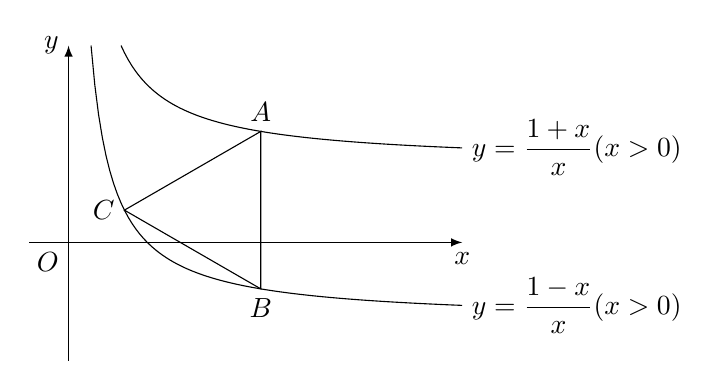
\begin{tikzpicture}[>=latex]
\draw [->] (-0.5,0) -- (5,0) node [below] {$x$};
\draw [->] (0,-1.5) -- (0,2.5) node [left] {$y$};
\draw (0,0) node [below left] {$O$};
\draw [domain = {2/7}:5, samples = 100] plot (\x,{(1-\x)/\x}) node [right] {$y=\dfrac{1-x}{x}$($x>0$)};
\draw [domain = {2/3}:5, samples = 100] plot (\x,{(1+\x)/\x}) node [right] {$y=\dfrac{1+x}{x}$($x>0$)};
\draw ({1/2*(sqrt(3)+sqrt(3+4*sqrt(3)))},{1/(1/2*(sqrt(3)+sqrt(3+4*sqrt(3))))}) ++ (0,1) node [above] {$A$} coordinate (A);
\draw (A) ++ (0,-2) node [below] {$B$} coordinate (B);
\draw (A) ++ (210:2) node [left] {$C$} coordinate (C);
\draw (A) -- (B) -- (C) -- cycle;
\end{tikzpicture}
\end{center}
\item 若$\overrightarrow a$与$\overrightarrow b-\overrightarrow c$都是非零向量, 则``$\overrightarrow a\cdot \overrightarrow b=\overrightarrow a\cdot \overrightarrow c$''是``$\overrightarrow a\perp (\overrightarrow b-\overrightarrow c)$''的\bracket{20}条件.
\fourch{充分不必要}{必要不充分}{充分必要}{既不充分也不必要}
\item 一个公司有$8$名员工, 其中$6$位员工的月工资分别为$5200$、$5300$、$5500$、$6100$、$6500$、$6600$, 另两位员工数据不清楚, 那么$8$位员工月工资的中位数不可能是\bracket{20}.
\fourch{$5800$}{$6000$}{$6200$}{$6400$}
\item 设$z_1,z_2$为复数, 则下列命题中一定成立的是\bracket{20}.
\twoch{如果$z_1-z_2>0$, 那么$z_1>z_2$}{如果$|z_1|=|z_2|$, 那么$z_1=\pm z_2$}{如果$|\dfrac{z_1}{z_2}|>1$, 那么$|z_1|>|z_2|$}{如果$z_1^2+z_2^2=0$, 那么$z_1=z_2=0$}
\item 对数列$\{a_n\}$, $\{b_n\}$, 若区间$[a_n,b_n]$满足下列条件: \textcircled{1} $[a_{n+1},b_{n+1}]\subseteq [a_n,b_n]$($n\in \mathbf{N}^*$); \textcircled{2} $\displaystyle\lim_{n\to\infty} (b_n-a_n)=0$, 
则称$\{[a_n,b_n]\}$为区间套, 并称$\{a_n\}$, $\{b_n\}$为区间套生成数列. 下列选项中, 是区间套生成数列的是\bracket{20}.
\twoch{$a_n=(\dfrac 12)^n$, $b_n=(\dfrac 23)^n$}{$a_n=(\dfrac 13)^n$, $b_n=\dfrac n{n^2+1}$}{$a_n=\dfrac{n-1}n$, $b_n=1+(\dfrac 13)^n$}{$a_n=\dfrac{n+3}{n+2}$, $b_n=\dfrac{n+2}{n+1}$}
\item 如图, 正四棱柱$ABCD-A_1B_1C_1D_1$的底面边长为$1$, 异面直线$AD$与$BC_1$所成角的大小为$60^\circ$, 求:
\begin{center}
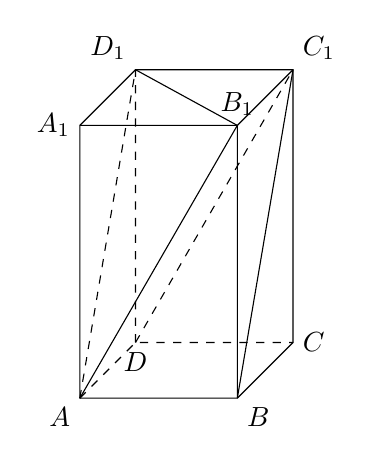
\begin{tikzpicture}[>=latex]
\draw (0,0) node [below left] {$A$} coordinate (A) --++ (2,0) node [below right] {$B$} coordinate (B) --++ (45:{2/2}) node [right] {$C$} coordinate (C)
--++ (0,{2*sqrt(3)}) node [above right] {$C_1$} coordinate (C1)
--++ (-2,0) node [above left] {$D_1$} coordinate (D1) --++ (225:{2/2}) node [left] {$A_1$} coordinate (A1) -- cycle;
\draw (A) ++ (2,{2*sqrt(3)}) node [above] {$B_1$} coordinate (B1) -- (B) (B1) --++ (45:{2/2}) (B1) --++ (-2,0);
\draw [dashed] (A) --++ (45:{2/2}) node [below] {$D$} coordinate (D) --++ (2,0) (D) --++ (0,{2*sqrt(3)});
\draw (B) -- (C1) (A) -- (B1) -- (D1);
\draw [dashed] (A) -- (D1) (D) -- (C1);
\end{tikzpicture}
\end{center}
(1) 线段$A_1B_1$到底面$ABCD$的距离;\\
(2) 三棱椎$B_1-ABC_1$的体积.
\item 已知函数$f(x)=2^x+\dfrac a{2^x}$, 其中$a$为实常数.\\
(1) 若$f(0)=7$, 解关于$x$的方程$f(x)=5$;\\
(2) 若对于任意的$x\in \mathbf{R}$, 恒有$f(x)\ge a$成立, 求$a$的取值范围.
\item 在上海世博会期间, 某工厂生产$A,B,C$三种世博纪念品, 每种纪念品均有精品型和普通型两种. 某一天产量如下表(单位:个):
\begin{center}
\begin{tabular}{|c|c|c|c|}
\hline
    & 纪念品$A$ & 纪念品$B$ & 纪念品$C$ \\ \hline
精品型 & $100$ & $150$ & $n$ \\ \hline
普通型 & $300$ & $450$ & $600$ \\ \hline
\end{tabular}
\end{center}
现采用分层抽样的方法在这一天生产的纪念品中抽取$200$个, 其中有$A$种纪念品$40$个.\\
(1)	求$n$的值;\\
(2)	从$B$种精品型纪念品中抽取$5$个, 其某种指标的数据分别如下: $x,y,10,11,9$. 把这$5$个数据看作一个总体, 其均值为$10$、方差为$2$, 求$|x-y|$的值;\\
(3)	用分层抽样的方法在$C$种纪念品中抽取一个容量为$5$的样本. 将该样本看成一个总体, 从中任取$2$个纪念品, 求至少有$1$个精品型纪念品的概率.
\item 如图, 在平面直角坐标系$xOy$中, 已知抛物线$C:y^2=4x$的焦点为$F$, 点$A$是第一象限内抛物线$C$上的一点, 点$D$的坐标为$(t,0)$($t>0$).
\begin{center}
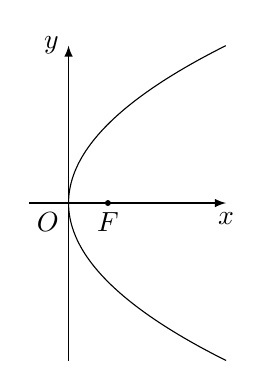
\begin{tikzpicture}[>=latex]
\draw [->] (-0.5,0) -- (2,0) node [below] {$x$};
\draw [->] (0,-2) -- (0,2) node [left] {$y$};
\draw (0,0) node [below left] {$O$};
\draw [domain = -2:2, samples = 100] plot ({pow(\x,2)/2},\x);
\filldraw (0.5,0) circle (0.03) node [below] {$F$};
\end{tikzpicture}
\end{center}
(1) 若$|OA|=\sqrt 5$, 求点$A$的坐标;\\
(2) 若$\triangle AFD$为等腰直角三角形, 且$\angle FAD=90^\circ$, 求点$D$的坐标;\\
(3) 弦$AB$经过点$D$, 过弦$AB$上一点$P$作直线$x=-t$的垂线, 垂足为点$Q$, 求证: ``直线$QA$与抛物线相切''的一个充要条件是``$P$为弦$AB$的中点''.
\item 已知无穷数列$\{a_n\}$的前$n$项和为$S_n$, 若对于任意的正整数$n$, 均有$S_{2n-1}\ge 0$, $S_{2n}\le 0$, 则称数列$\{a_n\}$具有性质$P$.\\
(1) 判断首项为$1$, 公比为$-2$的无穷等比数列$\{a_n\}$是否具有性质$P$, 并说明理由;\\
(2) 已知无穷数列$\{a_n\}$具有性质$P$, 且任意相邻四项之和都相等, 求证: $S_4=0$;\\
(3) 已知$b_n=2n-1$($n\in \mathbf{N}^*$), 数列$\{c_n\}$是等差数列, $a_n=\begin{cases}   b_{\frac{n+1}2}, & n\text{为奇数},  \\c_{\frac n2}, &  n\text{为偶数}.  \end{cases}$ 若无穷数列$\{a_n\}$具有性质$P$, 求$c_{2021}$的取值范围.


%zmj12
\item 不等式$\dfrac 1x<1$的解集为\blank{50}.
\item 抛物线$y^2=2x$的焦点坐标为\blank{50}.
\item 三阶行列式$\begin{vmatrix}
3 & -5 & 1  \\ 2 & 3 & -6  \\ -7 & 2 & 4  \end{vmatrix}$中元素$-5$的代数余子式的值为\blank{50}.
\item 已知向量$\overrightarrow a=(1,-2)$, $\overrightarrow b=(3,4)$, 则向量$\overrightarrow a$在向量$\overrightarrow b$的方向上的投影为\blank{50}.
\item 已知数列$\{a_n\}$为等差数列, 其前$n$项和为$S_n$.若$S_9=36$, 则$a_3+a_4+a_8=$\blank{50}.
\item 已知直线$l:x-y+b=0$被圆$C:x^2+y^2=25$所截得的弦长为$6$, 则$b=$\blank{50}.
\item 已知函数$y=f(x)$是定义在$\mathbf{R}$上的偶函数, 且在$[0,+\infty)$上是增函数, 若$f(a+1)\le f(4)$, 则实数$a$的取值范围是\blank{50}.
\item 函数$f(x)=(\sqrt 3\sin x+\cos x)(\sqrt 3\cos x-\sin x)$的最小正周期为\blank{50}.
\item 过双曲线$C:\dfrac{x^2}{a^2}-\dfrac{y^2}4=1$的右焦点$F$作一条垂直于$x$轴的垂线交双曲线$C$的两条渐近线于$A$、$B$两点, $O$为坐标原点, 则$\triangle OAB$的面积的最小值为\blank{50}.
\item 若关于$x$的不等式$|2^x-m|-\dfrac 1{2^x}<0$在区间$[0,1]$内恒成立, 则实数$m$的范围是\blank{50}.
\item 已知数列$\{a_n\}$满足: $na_{n+2}=1007(n-1)a_{n+1}+2018(n+1)a_n(n\in \mathbf{N}^*)$, 且$a_1=1,a_2=2,$若$\displaystyle\lim_{n\to\infty} \dfrac{a_{n+1}}{a_n}=A,$则$A=$\blank{50}.
\item 已知函数$f(x)=\begin{cases} \dfrac x{4x^2+16}, & x\ge 2, \\ (\dfrac 12)^{|x-a|}, & x<2, \end{cases}$ 若对任意的$x_1\in [2,+\infty)$, 都存在唯一的$x_2\in (-\infty ,2)$, 满足$f(x_1)=f(x_2)$, 则实数$a$的取值范围为\blank{50}.
\item 若实数$x,y\in \mathbf{R}$, 则陈述句甲``$\begin{cases} x+y>4, \\ xy>4 \end{cases}$''是陈述句乙``$\begin{cases} x>2, \\ y>2 \end{cases}$''的\bracket{20}条件.
\fourch{充分非必要}{必要非充分}{充要}{既非充分又非必要}
\item 已知$\triangle ABC$中, $\angle A=\dfrac{\pi }2$, $AB=AC=1$, 点$P$是$AB$边上的动点, 点$Q$是$AC$边上的动点, 则$\overrightarrow{BQ}\cdot \overrightarrow{CP}$的最小值为\bracket{20}.
\fourch{$-4$}{$-2$}{$-1$}{$0$}
\item 设$\{a_n\}$是等差数列, 下列命题中正确的是\bracket{20}.
\twoch{若$a_1+a_2>0$, 则$a_2+a_3>0$}{若$a_1+a_3<0$, 则$a_1+a_2<0$}{若$0<a_1<a_2$, 则$a_2>\sqrt {a_1a_3}$}{若$a_1<0$, 则$(a_2-a_1)(a_2-a_3)>0$}
\item 已知点$A(1,-2)$, $B(2,0)$, $P$为曲线$y=\sqrt {3-\dfrac 34x^2}$上任意一点, 则$\overrightarrow{AP}\cdot \overrightarrow{AB}$的取值范围为\bracket{20}.
\fourch{$[1,7]$}{$[-1,7]$}{$[1,3+2\sqrt 3]$}{$[-1,3+2\sqrt 3]$}
\item 如图, 四棱锥$S-ABCD$的底面是正方形, $SD \perp$平面$ABCD$, $SD=AD=2$.
\begin{center}
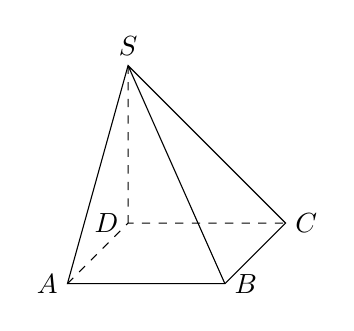
\begin{tikzpicture}[>=latex]
\draw (0,0,0) node [left] {$D$} coordinate (D);
\draw (2,0,0) node [right] {$C$} coordinate (C);
\draw (2,0,2) node [right] {$B$} coordinate (B);
\draw (0,0,2) node [left] {$A$} coordinate (A);
\draw (0,2,0) node [above] {$S$} coordinate (S);
\draw (S) -- (A) -- (B) -- (C) -- cycle (S) -- (B);
\draw [dashed] (A) -- (D) -- (C) (S) -- (D);
\end{tikzpicture}
\end{center}
(1) 求证: $AC\perp SB$;\\
(2) 求二面角$C-SA-D$的大小.
\item 已知函数$f(x)=2\sqrt 3\sin x\cos x-2\sin ^2x$.\\
(1) 若角$\alpha$的终边与单位圆交于点$P(\dfrac 35,\dfrac 45)$, 求$f(\alpha)$的值;\\
(2) 当$x\in [-\dfrac{\pi }6, \dfrac{\pi }3]$时, 求$f(x)$的单调递增区间和值域.
\item 设数列$\{a_n\}$满足$a_{n+1}=2a_n+n^2-4n+1$, $b_n=a_n+n^2-2n$.\\
(1) 若$a_1=2$, 求证: 数列$\{b_n\}$为等比数列;\\
(2) 在(1)的条件下, 对于正整数$2$、$q$、$r$($2<q<r$), 若$5b_2$、$b_q$、$b_r$这三项经适当排序后能构成等差数列, 求符合条件的数组$(q,r)$.
\item 已知双曲线$\Gamma$: $\dfrac{x^2}{a^2}-\dfrac{y^2}{b^2}=1$($a>0$, $b>0$)的左、右焦点分别是 $F_1$、$F_2$, 左、右两顶点分别是 $A_1$、$A_2$, 弦$AB$和$CD$所在直线分别平行于$x$轴与$y$轴, 线段$BA$的延长线与线段$CD$相交于点$P$(如图).
\begin{center}
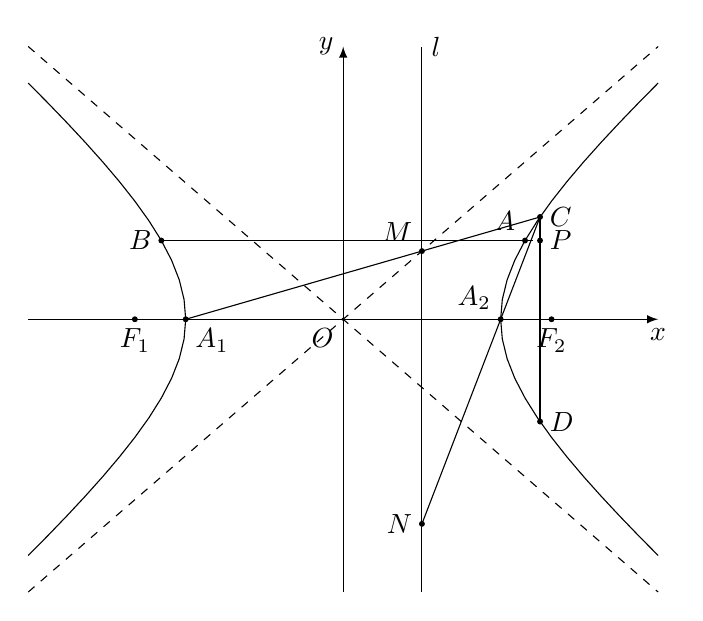
\begin{tikzpicture}[>=latex]
\draw [->] (-4,0) -- (4,0) node [below] {$x$};
\draw [->] (0,{-2*sqrt(3)}) -- (0,{2*sqrt(3)}) node [left] {$y$};
\draw (0,0) node [below left] {$O$};
\draw [domain = -3:3] plot ({2*sqrt(pow(\x,2)/3+1)},\x);
\draw [domain = -3:3] plot ({-2*sqrt(pow(\x,2)/3+1)},\x);
\draw [dashed] (-4,{-2*sqrt(3)}) -- (4,{2*sqrt(3)}) (-4,{2*sqrt(3)}) -- (4,{-2*sqrt(3)});
\draw (1,{-2*sqrt(3)}) -- (1,{2*sqrt(3)}) node [right] {$l$};
\filldraw ({-sqrt(7)},0) circle (0.03) node [below] {$F_1$} ({sqrt(7)},0) circle (0.03) node [below] {$F_2$};
\filldraw (-2,0) circle (0.03) node [below right] {$A_1$} coordinate (A1) (2,0) circle (0.03) node [above left] {$A_2$} coordinate (A2);
\draw ({-4/sqrt(3)},1) node [left] {$B$} coordinate (B) -- ({4/sqrt(3)},1) node [above left] {$A$} coordinate (A);
\draw [dashed] (A) -- (2.5,1) node [right] {$P$} coordinate (P);
\draw (2.5,{-3*sqrt(3)/4}) node [right] {$D$} coordinate (D) -- (2.5,{3*sqrt(3)/4}) node [right] {$C$} coordinate (C);
\draw (C) -- (A1) (C) -- ($(C)!3!(A2)$) node [left] {$N$} coordinate (N) ($(C)!{1.5/4.5}!(A1)$) node [above left] {$M$} coordinate (M);
\filldraw (C) circle (0.03) (D) circle (0.03) (M) circle (0.03) (N) circle (0.03) (A) circle (0.03) (B) circle (0.03) (P) circle (0.03);
\end{tikzpicture}
\end{center}
(1) 若$\overrightarrow d=(2,\sqrt 3)$是$\Gamma$的一条渐近线的一个方向向量, 试求$\Gamma$的两渐近线的夹角$\theta$;\\
(2) 若$|PA|=1$, $|PB|=5$ , $|PC|=2$, $|PD|=4$, 试求双曲线$\Gamma$的方程;\\
(3) 在(1)的条件下, 且$|A_1A_2|=4$, 点$C$与双曲线的顶点不重合, 直线$CA_1$和直线$CA_2$与直线$l:x=1$分别相交于点$M$和$N$, 试问: 以线段$MN$为直径的圆是否恒经过定点? 若是, 请求出定点的坐标; 若不是, 试说明理由.
\item 已知平面直角坐标系$xOy$, 在$x$轴的正半轴上, 依次取点$A_1,A_2,A_3,\cdots,A_n$($n\in \mathbf{N}^*$), 并在第一象限内的抛物线$y^2=\dfrac 32x$上依次取点$B_1,B_2,B_3,\cdots ,B_n$($n\in \mathbf{N}^*$), 使得$\triangle A_{k-1}B_kA_k(k\in \mathbf{N}^*)$都为等边三角形, 其中$A_0$为坐标原点, 设第$n$个三角形的边长为$f(n)$.\\
(1) 求$f(1),f(2)$, 并猜想$f(n)$(不要求证明);\\
(2) 令$a_n=9f(n)-8$, 记$t_m$为数列$\{a_n\}$中落在区间$(9^m,9^{2m})$内的项的个数, 设数列$\{t_m\}$的前$m$项和为$S_m$, 试问是否存在实数$\lambda$, 使得$2^{\lambda }\le S_m$对任意$m\in \mathbf{N}^*$恒成立? 若存在, 求出$\lambda$的取值范围; 若不存在, 说明理由;\\
(3) 已知数列$\{b_n\}$满足: $b_1=\dfrac{\sqrt 2}2$, $b_{n+1}=\dfrac{\sqrt 2}2\sqrt {1-\sqrt {1-b_n^2}}$, 数列$\{c_n\}$满足: $c_1=1$, $c_{n+1}=\dfrac{\sqrt {1+c_n^2}-1}{c_n}$, 求证: $b_n<\dfrac{\pi }{2^{n+1}}<c_n$.


%zmj8
\item 已知集合$A=\{1,2,m\}$, $B=\{3,4\}$, 若$A\cap B=\{4\}$, 则实数$m=$\blank{50}
\item 若$\mathrm{P}_n^2=6$, 则$n=$\blank{50}.
\item 函数$f(x)=\arcsin x+1$的定义域为\blank{50}.
\item 若球的大圆的面积为$9\pi$, 则该球的体积为\blank{50}.
\item 函数$f(x)=\sin^2 x-\cos^2 x$的最小正周期为\blank{50}.
\item 若掷一颗质地均匀的骰子, 则出现向上的点数大于$4$的概率是\blank{50}.
\item 若$f(x)=\sin x\cos \theta+\cos x\sin\theta$是定义在$\mathbf{R}$上的偶函数, 其中$0\le \theta\le \dfrac \pi 2$, 则$\theta=$\blank{50}.
\item 设常数$a\in \mathbf{R}$, 函数$f(x)=\ln (x+a)$. 若$f(x)$的反函数图像经过点$(3,1)$, 则$a=$\blank{50}.
\item 函数$y=\sqrt{x}-\sqrt{1-x}$的值域为\blank{50}.
\item 若非零实数$a,b$满足$a^2+4b^2=1$, 则$\dfrac{2ab}{|a|+2|b|}$的最大值为\blank{50}.
\item 已知$f(x)$是定义域为$\mathbf{R}$的奇函数, 满足$f(1+x)=f(1-x)$. 若$f(1)=2$, 则$f(1)+f(2)+f(3)+\cdots+f(2018)=$\blank{50}.
\item 已知定义域为$(0,+\infty)$的函数$f(x)$满足: 对任何$x\in (0,+\infty)$, 都有$f(3x)=3f(x)$, 且当$x\in (1,3]$时, $f(x)=3-x$. 在下列结论中, 正确命题的序号是\blank{50}.\\
\textcircled{1} 对任何$m\in \mathbf{Z}$, 都有$f(3^m)=0$; \textcircled{2} 函数$f(x)$的值域是$[0,+\infty)$; \textcircled{3} 存在$n\in \mathbf{Z}$, 使得$f(3^n+1)=17$; \textcircled{4} ``函数$f(x)$在区间$(a,b)$上单调递减''的一个充要条件是``存在$k\in \mathbf{Z}$, 使得$(a,b)\subseteq (3^k,3^{k+1})$''.
\item 为了得到函数$y=\sin(x+\dfrac {5\pi}{6})$的图像, 可将函数$y=\sin x$的图像\bracket{20}.
\fourch{左移$\dfrac{5\pi}6$个长度}{右移$\dfrac{5\pi}6$个长度}{左移$\dfrac{5\pi}{12}$个长度}{右移$\dfrac{5\pi}{12}$个长度}
\item 已知$a,b\in \mathbf{R}$, 则``$ab>0$''是``$\dfrac ab+\dfrac ba>2$''的\bracket{20}.
\twoch{充分非必要条件}{必要非充分条件}{充要条件}{既非充分也非必要条件}
\item 符号$[x]$表示不超过$x$的最大整数, 如$[\pi]=3$, $[-1.08]=-2$, 定义函数$\{x\}=x-[x]$, 那么下列命题中正确的序号是\bracket{20}.\\
\textcircled{1} 函数$\{x\}$的定义域为$\mathbf{R}$, 值域为$[0,1]$; \textcircled{2} 方程$\{x\}=\dfrac 12$有无数解; \textcircled{3} 函数$\{x\}$是周期函数; \textcircled{4} 函数$\{x\}$是增函数.
\fourch{\textcircled{1}\textcircled{2}}{\textcircled{3}\textcircled{3}}{\textcircled{3}\textcircled{4}}{\textcircled{4}\textcircled{1}}
\item 如图所示, 已知$PA\perp$平面$ABC$, $AD\perp BC$于$D$, $BC=CD=AD=1$. 令$PD=x$, $\angle BPC=\theta$, 则\bracket{20}.
\begin{center}
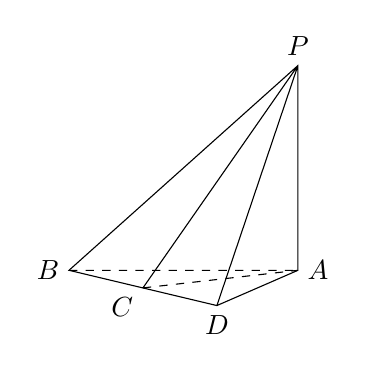
\begin{tikzpicture}[>=latex,scale = 1.3]
\draw (0,0,0) node [right] {$A$} coordinate (A);
\draw ({-sqrt(5)},0,0) node [left] {$B$} coordinate (B);
\draw ($(A)!0.2!(B)$) ++ (0,0,{2/sqrt(5)}) node [below] {$D$} coordinate (D);
\draw ($(B)!0.5!(D)$) node [below left] {$C$} coordinate (C);
\draw (A) ++ (0,2,0) node [above] {$P$} coordinate (P);
\draw (B) -- (D) -- (A) -- (P) -- cycle (P) -- (C) (P) -- (D);
\draw [dashed] (B) -- (A) (C) -- (A);
\end{tikzpicture}
\end{center}
\fourch{$\tan\theta = \dfrac{x}{x^2+2}$}{$\tan\theta = \dfrac{x}{x^2+1}$}{$\tan\theta=\dfrac{1}{x^2+2}$}{$\tan\theta=\dfrac{1}{x^2+1}$}
\item 在$\triangle ABC$中, 角$A,B,C$所对的边分别为$a,b,c$. $b=\sqrt{5}$, $B=\dfrac{\pi}{4}$.\\
(1) 若$a=3$, 求$\sin A$的值;\\
(2) 若$\triangle ABC$的面积等于$1$, 求$a$的值.
\item 如图, 圆锥的顶点是$P$, 底面中心是$O$, 已知$OP=\sqrt{2}$, 圆$O$的直径是$AB=2$, 点$C$在弧$AB$上, 且$\angle CAB=30^\circ$.
\begin{center}
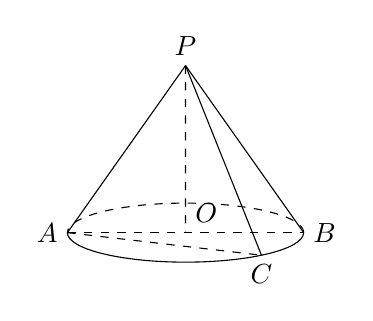
\begin{tikzpicture}[>=latex, scale = 1.5]
\draw (0,0) node [above right] {$O$} coordinate (O);
\draw [dashed] (-1,0) node [left] {$A$} coordinate (A) -- (1,0) node [right] {$B$} coordinate (B);
\draw (0,{sqrt(2)}) node [above] {$P$} coordinate (P);
\draw (P) -- (A) (P) -- (B);
\draw (A) arc (180:360:1 and 0.25);
\draw (B) [dashed] arc (0:180:1 and 0.25) (P) -- (O);
\draw ({cos(-50)},{0.25*sin(-50)}) node [below] {$C$} coordinate (C);
\draw (C) -- (P);
\draw [dashed] (A) -- (C);
\end{tikzpicture}
\end{center}
(1) 求圆锥的侧面积;\\
(2) 求$O$到平面$APC$的距离.
\item 科学家发现某种特别物质的温度$y$(单位: 摄氏度)随时间$=$x$($时间:分钟)的变化规律满足关系式: $y=m2^x+2^{1-x}$, ($0\le x\le 4$, $m>0$).\\
(1) 若$m=2$, 求经过多少分钟, 该物质的温度为$5$摄氏度;\\
(2) 如果该物质温度总不低于$2$摄氏度, 求$m$的取值范围.
\item 已知函数$f(x)=\log_2(a x^2+2x-a)$.\\
(1) 当$a=-1$时, 求该函数的定义域;\\
(2) 当$a\le 0$时, 如果$f(x)\ge 1$对任何$x\in [2,3]$都成立, 求实数$a$的取值范围;\\
(3) 若$a<0$, 将函数$f(x)$的图像沿$x$轴或其相反方向平移, 得到一个偶函数$g(x)$的图像, 设函数$g(x)$的最大值为$h(a)$, 求$h(a)$的最小值.
\item 记$f_k(x)=x^k$($x>0$, $k\in \mathbf{Z}$).\\
(1) 求函数$F(x)=f_2(x-1)-1$的零点;\\
(2) 设$\xi,\eta,\mu$均为正整数, 且$\sqrt{\mu}$为最简根式, 若存在$n_0\in \mathbf{N}^*$, 使得$f_{n_0}(\xi+\eta\sqrt{\mu})$可唯一表示为$\sqrt{\tau}+\sqrt{\tau-1}$的形式($\tau\in\mathbf{N}^*$). 求证: $|\xi^2-\eta^2\mu|=1$;\\
(3) 已知$f_{-1}(t)+f_{-1}(s)=1$, 是否存在$n_1\in \mathbf{N}^*$, 使得$\dfrac{f_{n_1}(t+2)-f_{n_1}(t)-f_{n_1}(s)+f_{n_1}(2)}{f_{n_1}(4)-f_{n_1}(2)}\ge 1$成立. 若存在, 试求出$n_1$的值; 若不存在, 请说明理由.

%zmj7
\item 函数$f(x)=\log_2(x-1)$的定义域为\blank{50}.
\item 已知集合$A=\{1,2,3,4\}$, 集合$B=\{4,5\}$, 则$A\cap B=$\blank{50}.
\item 函数$y=2\cos ^2x-1$的最小正周期为\blank{50}. 	
\item 已知球的体积为$36\pi$, 则该球大圆的面积等于\blank{50}.
\item 二项式$(x-\dfrac 1x)^6$的展开式中的常数项为\blank{50}. (用数字作答)
\item 若圆锥的母线长$l=5(\text{cm})$, 高$h=4(\text{cm})$, 则这个圆锥的体积为\blank{50}$(\text{cm}^3)$.
\item 已知函数$f(x)=a^{x+1}-2$($a>0$且$a\ne 1$), 设$f^{-1}(x)$是$f(x)$的反函数. 若$y=f^{-1}(x)$的图象不经过第二象限, 则$a$的取值范围为\blank{50}.
\item 函数$f(x)=2\sin (\omega x+\varphi)$($\omega >0$)的部分图像, 如图所示, 若$|AB|=5$, 则$\omega$的值为\blank{50}.
\begin{center}
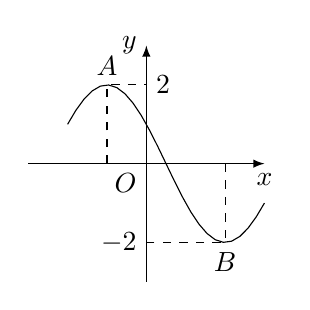
\begin{tikzpicture}[>=latex,scale = 0.5]
\draw [->] (-3,0) -- (3,0) node [below] {$x$};
\draw [->] (0,-3) -- (0,3) node [left] {$y$};
\draw (0,0) node [below left] {$O$};
\draw [domain = -2:3] plot (\x,{2*sin(pi/3*\x/pi*180+150)});
\draw [dashed] (-1,0) -- (-1,2) node [above] {$A$} coordinate (A) -- (0,2) node [right] {$2$};
\draw [dashed] (2,0) -- (2,-2) node [below] {$B$} coordinate (B) -- (0,-2) node [left] {$-2$};
\end{tikzpicture}
\end{center}
\item 在$100$件产品中有$90$件一等品, $10$件二等品, 从中随机取出$4$件产品.
则恰含$1$件二等品的概率是\blank{50}. (结果精确到$0.01$)
\item 已知函数$f(x)=\log_a(x+b)$($a>0$, $a\ne 1$, $b\in \mathbf{R}$)的图像, 如图所示, 则$a+b$的值是\blank{50}.
\begin{center}
\begin{tikzpicture}[>=latex, scale = 0.5]
\draw [->] (-4,0) -- (4,0) node [below] {$x$};
\draw [->] (0,-3) -- (0,3) node [left] {$y$};
\draw (0,0) node [below left] {$O$};
\draw [domain = -3.5:4, samples = 100] plot (\x,{ln(\x+4)/ln(0.5)});
\draw (-3,0) node [below left] {$-3$} (0,-2) node [below left] {$-2$};
\end{tikzpicture}
\end{center}
\item 函数$F(x)=\lg x-\sin x$零点的个数是\blank{50}个.
\item 设函数$f(x)$和$g(x)$都是定义在集合$M$上的函数, 若对于任意$x\in M$, 都有$f(g(x))=g(f(x))$成立, 就称函数$f(x)$与$g(x)$在$M$上互为``互换函数''.若存在非空集合$M$, 使得函数$f(x)=a^x$($a>0$, $a\ne 1$)与$g(x)=x+1$在集合$M$上互为``互换函数'', 则实数$a$的取值范围是\blank{50}.
\item 函数$f(x)=2^x-\dfrac 1{2^x}$的图像关于\bracket{20}.
\fourch{原点对称}{直线$y=x$对称}{直线$y=-x$对称}{$y$轴对称}
\item 三国时期赵爽在《勾股方圆图注》中, 对勾股定理的证明可用现代数学表述为如图所示, 可以利用该图作为几何解释的不等式性质是\bracket{20}.
\begin{center}
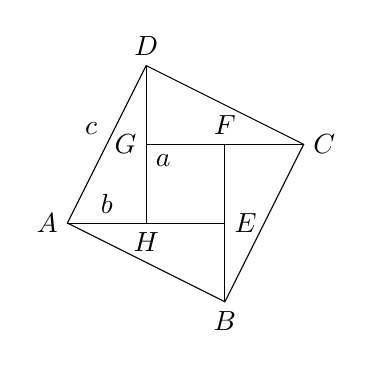
\begin{tikzpicture}[>=latex]
\draw (0,0) node [left] {$A$} coordinate (A) -- (2,0) node [right] {$E$};
\draw (1,0) node [below] {$H$} -- (1,2) node [above] {$D$} coordinate (D);
\draw (1,1) node [left] {$G$} -- (3,1) node [right] {$C$} coordinate (C);
\draw (2,1) node [above] {$F$} -- (2,-1) node [below] {$B$} coordinate (B);
\draw (A) -- (D) -- (C) -- (B) -- cycle;
\draw (0.5,0) node [above] {$b$} (1,1) node [below right] {$a$} ($(A)!0.5!(D)$) node [above left] {$c$};
\end{tikzpicture}
\end{center}
\onech{如果$a>b$, $b>c$, 那么$a>c$}{如果$a>b>0$, 那么$a^2>b^2$}{对任意正实数$a$和$b$, 有$a^2+b^2\ge 2ab$, 当且仅当$a=b$时等号成立}{如果$a>b$, $c>0$, 那么$ac>bc$}
\item 若函数$f(x)=\begin{cases} \log_2x, & x\ge 1, \\ x+c, & x<1. \end{cases}$  则``$c=-1$''是``$y=f(x)$是$\mathbf{R}$上的单调增函数''的\bracket{20}.
\twoch{充分非必要条件}{必要非充分条件}{充要条件}{既非充分也非必要条件}
\item 若实数$x,y$满足$x^2+2\cos y=1$, 则$x-\cos y$的取值范围是\bracket{20}.
\fourch{$[-1,\sqrt{3}+1)$}{$[-1,\sqrt 3]$}{$[1,\sqrt 3+1)$}{$[-1,\sqrt 3+1]$}
\item 如图, 正四棱柱$ABCD-A_1B_1C_1D_1$的底面边长$AB=2$, 异面直线$A_1A$与$B_1C$所成角的大小为$\arctan \dfrac 12$.
\begin{center}
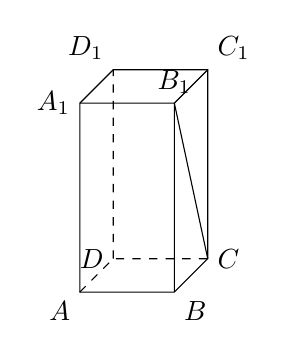
\begin{tikzpicture}[>=latex,scale = 0.6]
\draw (0,0) node [below left] {$A$} coordinate (A) --++ (2,0) node [below right] {$B$} coordinate (B) --++ (45:{2/2}) node [right] {$C$} coordinate (C)
--++ (0,4) node [above right] {$C_1$} coordinate (C1)
--++ (-2,0) node [above left] {$D_1$} coordinate (D1) --++ (225:{2/2}) node [left] {$A_1$} coordinate (A1) -- cycle;
\draw (A) ++ (2,4) node [above] {$B_1$} coordinate (B1) -- (B) (B1) --++ (45:{2/2}) (B1) --++ (-2,0);
\draw [dashed] (A) --++ (45:{2/2}) node [left] {$D$} coordinate (D) --++ (2,0) (D) --++ (0,4);
\draw (C) -- (B1);
\end{tikzpicture}
\end{center}
(1) 求$BD_1$与底面$ABCD$所成角的正切值;\\
(2) 求正四棱柱$ABCD-A_1B_1C_1D_1$的体积.
\item 在$\triangle ABC$中, 内角$A,B,C$所对的边长分别是$a,b,c$.\\
(1) 若$c=2$, $C=\dfrac{\pi }3$, 且$\triangle ABC$的面积$S=\sqrt 3$, 求$a,b$的值;\\
(2) 若$\sin (A+B)+\sin (B-A)=\sin 2A$, 试判断$\triangle ABC$的形状.
\item 如图, 某班级墙上有一壁画, 最高点$A$离地面$4$米, 最低点$B$离地面$2$米, 某同学从距离墙$x$($x>1$)米, 离地面高$a$($1\le a\le 2$)米的$C$处观赏该壁画, 设观赏视角$\angle ACB=\theta$.
\begin{center}
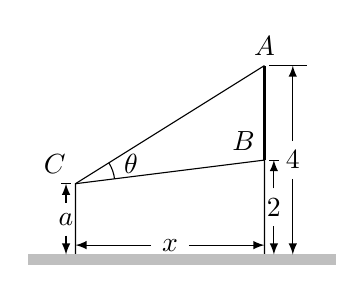
\begin{tikzpicture}[>=latex,scale = 0.6]
\draw (0,0) -- (0,1.5) node [above left] {$C$} coordinate (C) -- (4,2) node [above left] {$B$} coordinate (B) ++ (0,2) node [above] {$A$} coordinate (A);
\draw [very thick] (B) -- (A);
\draw (C) -- (A) (B) --++ (0,-2);
\draw (C) pic ["$\theta$", draw, angle eccentricity = 1.5] {angle = B--C--A};
\filldraw [gray!50] (-1,0) rectangle (5.5,-0.2);
\draw (-0.1,1.5) -- (-0.3,1.5);
\draw [->] (-0.2,1.1) -- (-0.2,1.5);
\draw [->] (-0.2,0.4) -- (-0.2,0);
\draw (-0.2,0.75) node {$a$};
\draw [->] (1.6,0.2) -- (0,0.2);
\draw [->] (2.4,0.2) -- (4,0.2);
\draw (2,0.2) node {$x$};
\draw (4.1,2) -- (4.3,2);
\draw [->] (4.2,0.6) -- (4.2,0);
\draw [->] (4.2,1.4) -- (4.2,2);
\draw (4.2,1) node {$2$};
\draw (4.1,4) -- (4.9,4);
\draw [->] (4.6,1.6) -- (4.6,0);
\draw [->] (4.6,2.4) -- (4.6,4);
\draw (4.6,2) node {$4$};
\end{tikzpicture}
\end{center}
(1) 若$a=1.5$米, 问该同学离墙多远时, 视角$\theta$最大;\\
(2) 若$\tan \theta =\dfrac 12$, 当$a$变化时, 求$x$的取值范围.
\item 已知函数$f(x)$的定义域是$\{x|x\in \mathbf{R},\ x\ne \dfrac k2, \ k\in \mathbf{Z}\}$, 且$f(x)+f(2-x)=0$, $f(x+1)=-\dfrac 1{f(x)}$, 当$0<x<\dfrac 12$时, $f(x)=3^x$.\\
(1) 判断$f(x)$的奇偶性, 并说明理由;\\
(2) 求$f(x)$在区间$(2k+\dfrac 12,2k+1)$($k\in \mathbf{Z}$)上的解析式;\\
(3) 是否存在整数$k$, 使得当$x\in (2k+\dfrac 12,2k+1)$时, 不等式$\log_3f(x)>x^2-k-1$有解? 证明你的结论.
\item 已知函数$f(x)=\ln (x^{-1}+a)$.\\
(1) 设$f^{-1}(x)$是$f(x)$的反函数. 当$a=1$时, 解不等式$f^{-1}(x)>0$;\\
(2) 若关于$x$的方程$f(x)+\ln (x^2)=0$的解集中恰好有一个元素, 求实数$a$的值;\\
(3) 设$a>0$, 若对任意$t\in [\dfrac 12,1]$, 函数$f(x)$在区间$[t,t+1]$上的最大值与最小值的差不超过$\ln 2$, 求$a$的取值范围.


\end{enumerate}

\iffalse
















































\fi




\end{document}